\documentclass{article}
\usepackage{graphicx} % Required for inserting images
\graphicspath{{./images/}} % Path to find images
\usepackage{multicol} % For double column in Appendix A 
\usepackage{geometry} 
\usepackage{amsfonts} % Required for \mathbb{} commands
\usepackage{amsmath} % So that I can embed text inside math mode using \text{} command as well as use {flalign} environment. Also used for matrices
\usepackage[table]{xcolor} % For table colours
\usepackage{float} % To enable [H] exact placement of table position
\usepackage{amssymb} % Allow me to use \therefore command in conclusion statements
\usepackage[mathscr]{euscript} % For curly C (set partition) symbol
\usepackage{xcolor, soul} % For text highlighting
\usepackage{tikz} % For graph drawings
\usepackage{pifont} % For star symbols \ding{73}

\title{Important Definitions for CS1231S}
\author{Michael Yang}
\date{Semester 1, AY23/24 (Prof Aaron Tan)}
\begin{document}
\maketitle
\newpage

% =================================== APPENDIX A ====================================== %

% Margins
\newgeometry{left=1cm, right=1cm, top=1cm, bottom=2cm}
\section*{Appendix A (Properties of Real Numbers)}
\hrule
\begin{multicols*}{2}
    \begin{description}
        \item[F1. Commutative Laws]For all real numbers $a$ and $b$, $a + b = b + a$ and $ab = ba$.
        \item[F2. Associative Laws]For all real numbers $a$, $b$ and $c$, $(a+b) + c = a + (b + c)$ and $(ab)c = a(bc)$.
        \item[F3. Distributive Laws]For all real numbers $a$, $b$ and $c$, $a(b + c) = ab + ac$ and $(b+c)a = ba + bc$.
        \item[F4. Existence of Identity Elements]There exists two distinct real numbers, denoted $0$ and $1$, such that for every real number $a$, $0 + a = a + 0$ and $1 \cdot a = a \cdot 1$.
        \item[F5. Existence of Additive Inverses]For every real number $a$, there is a real number, denoted $-a$ and called the \textbf{additive inverse} of $a$, such that $a + (-a) = (-a) + a = 0$.
        \item[F6. Existence of Reciprocals]For every real number $a\neq0$, there is a real number, denoted $1/a$ or $a^{-1}$, called the \textbf{reciprocal} of $a$, such that $a \cdot (\frac{1}{a}) = (\frac{1}{a})\cdot a = 1$.
        \item[T1. Cancellation Law for Addition]If $a + b = a + c$ , then $b = c$. (In particular, this shows that the number 0 of Axiom F4 is unique.)
        \item[T2. Possibility of Subtraction]Given $a$ and $b$, there is exactly one $x$ such that $a+x=b$. This $x$ is denoted by $b-a$. In particular, $0-a$ is the additive inverse of $a$, $-a$.
        \item[T3.]$b-a=b+(-a)$.
        \item[T4.]$-(-a)=a$.
        \item[T5.]$a(b-c)=ab-ac$.
        \item[T6.]$0\cdot a=a\cdot0=0$.
        \item[T7. Cancellation Law for Multiplication] If $ab=bc$ and $a\neq0$, then $b=c$. (In particular, this shows that the number 1 of Axiom F4 is unique.)
        \item[T8. Possibility of Division]Given $a$ and $b$ with $a\neq0$, there is exactly one $x$ such that $ax=b$. This $x$ is denoted by $b/a$ and is called the \textbf{quotient} of $b$ and $a$. In particular, $1/a$ is the reciprocal of $a$.
        \item[T9.]If $a\neq0$, then $b/a=b\cdot a^{-1}$.
        \item[T10.]If $a\neq0$, then $(a^{-1})^{-1}=a$.
        \item[T11. Zero Product Property]If $ab=0$, then $a=0$ or $b=0$. 
        \item[T12. Rule for Multiplication with Negative Signs]$(-a)b=a(-b)=-(ab)$, and $-\frac{a}{b}=\frac{-a}{b}=\frac{a}{-b}$.
        \item[T13. Equivalent Fractions Property]$\frac{a}{b}=\frac{ac}{bc}$, if $b\neq0$ and $c\neq0$.
        \item[T14. Rule for Addition of Fractions]$\frac{a}{b}+\frac{c}{d}=\frac{ad+bc}{bd}$, if $b\neq0$ and $d\neq0$.
        \item[T15. Rule for Multiplication of Fractions]$\frac{a}{b}\cdot\frac{c}{d}=\frac{ac}{bd}$, if $b\neq0$ and $d\neq0$.
        \item[T16. Rule for Division of Fractions]$\frac{a}{b}\div\frac{c}{d}=\frac{ad}{bc}$, if $b\neq0$, $c\neq0$ and $d\neq0$.
        \item[T17. Trichotomy Law]For arbitrary real numbers $a$ and $b$, exactly one of these three relations $a<b$, $b>a$ or $a=b$ holds. 
        \item[T18. Transitive Law]If $a<b$ and $b<c$, then $a<c$.
        \item[T19.]If $a<b$, then $a+c<b+c$.
        \item[T20.]If $a<b$ and $c>0$, then $ac<bc$.
        \item[T21.]If $a\neq0$, then $a^2>0$.
        \item[T22.]$1>0$.
        \item[T23.]If $a<b$ and $c<0$, then $ac>bc$.
        \item[T24.]If $a<b$, then $-a>-b$. In particular, if $a<0$, then $-a>0$.
        \item[T25.]If $ab>0$, then both $a$ and $b$ are positive or both are negative.
        \item[T26.]If $a<c$ and $b<d$, then $a+b<c+d$.
        \item[T27.]If $0<a<c$ and $0<b<d$, then $0<ab<cd$.
        \item[Ord1.]For any real numbers $a$ and $b$, if $a$ and $b$ are positive, so are $a+b$ and $ab$. 
        \item[Ord2.]For every real number $a\neq 0$, either $a$ is positive or $-a$ is positive but not both.
        \item[Ord3.]The number 0 is not positive. 
        \item[Definition]Given real numbers $a$ and $b$, $a < b$ means $b + (-a)$ is positive. $b > a$ means $a < b$. $a\leq b$ means $a < b$ or $a=b$. $b\geq a$ means $a\leq b$. If $a < 0$, we say that $a$ is \textbf{negative}. If $a \geq 0$, we say that $a$ is \textbf{non-negative}.
    \end{description}
    \hrule

    \paragraph{Note:} Whenever you are proving a universal statement using an arbitrary particular, you should quote \textbf{WLOG} (Without Loss Of Generality). This means that the proof for the special case can be easily applied to all other cases. 
\end{multicols*}

% ==================================== DEFINITIONS =====================================

\newcommand{\iterate}[2]{$#1_{1}, #1_{2},\dots,#1_{#2}$} % Makes iterating over elements easy i.e. v1, v2, ... vn. Usage: \iterate{v}{n} - v is the element you want to iterate, n is the endpoint (inclusive)

\newpage
\section*{Definitions}
\hrule
\vspace{0.3cm}
\begin{description}
    \item[Divisibility] If $n,d\in\mathbb{Z}$ and $d\neq0$, $d\vert{n}\Leftrightarrow \exists{k} \in \mathbb{Z}$ such that $n=dk$.
    \item[Rational Numbers]$r$ is rational $\leftrightarrow \exists a,b\in\mathbb{Z}$ s.t. $r=\frac{a}{b}$ and $b\neq0$.
    \item[Fraction in lowest term]A fraction $\frac{a}{b}$ where $b\neq0$ is said to be in \textbf{lowest terms} if the largest integer that divides both $a$ and $b$ is 1. 
    \item[Prime and Composite] An integer $n$ is \textbf{prime} iff $n > 1$ and for all positive integers $r$ and $s$, if $n=rs$, then either $r$ or $s$ equals $n$. An integer $n$ is \textbf{composite} iff $n >  1$ and $n=rs$ for some integers $r$ and $s$ with $1 < r < n$ and $1 < s < n$. In symbols, 
    \begin{description}
		\item[$n$ is prime:] $(n > 1) \land \forall r, s\in \mathbb{Z}^{+}$, $(n=rs\to (r=1\land s=n) \lor (r=n\land s=1))$. 
		\item[$n$ is composite:] $\exists r, s\in \mathbb{Z}^{+} (n=rs\land (1 < r < n) \land (1 < s < n))$.
    \end{description}
        
    % 2 - Compound Statements
    \vspace{0.2cm}
    \item[\large Compound Statements]
    \item[2.1.1 Statement]A \textbf{statement} (or \textbf{proposition}) is a sentence that is true or false, but not both.
    \item[2.1.2 Negation]If $p$ is a variable, the \textbf{negation} of $p$ is "not $p$" or it is not the case that $p$" and is denoted ${\sim}p$. 
    \item[2.1.3 Conjunction]If $p$ and $q$ are statement variables, the conjunction of $p$ and $q$ is ``$p$ and $q$'', denoted $p \wedge q$.
    \item[2.1.4 Disjunction]If $p$ and $q$ are statement variables, the disjunction of $p$ and $q$ is “$p$ or $q$”, denoted $p \vee q$.
    \item[2.1.5 Statement Form]A statement form (or propositional form) is an expression made up of statement variables and logical connectives that becomes a statement when actual statements are substituted for the component statement variables.
    \item[2.1.6 Logical Equivalence]Two statement forms are called logically equivalent if, and only if, they have identical truth values for each possible substitution of statements for their statement variables. The logical equivalence of statement forms $P$ and $Q$ is denoted by $P \equiv Q$.
    \item[2.1.7 Tautology]A tautology is a statement form that is \textbf{always true} regardless of the truth values of the individual statements substituted for its statement variables. A statement whose form is a tautology is a \textbf{tautological statement}.
    \item[2.1.8 Contradiction]A contradiction is a statement form that is \textbf{always false} regardless of the truth values of the individual statements substituted for its statement variables. A statement whose form is a contradiction is a \textbf{contradictory statement}. 
    \item[2.2.1 Conditional]If $p$ and $q$ are statement variables, the conditional of $q$ by $p$ is “if $p$ then $q$” or “$p$ implies $q$”, denoted $p\to q$. It is false when p is true and q is false; otherwise it is true. We called $p$ the \textbf{hypothesis} (or \textbf{antecedent}) of the conditional and $q$ the \textbf{conclusion} (or \textbf{consequent}).
    \item[2.2.2 Contrapositive] The contrapositive of a conditional statement of the form “if $p$ then $q$” is ``if ${\sim} q$ then ${\sim} p$''. Symbolically, the contrapositive of $p\to q$ is ${\sim} q\to {\sim} p$.
    \item[2.2.3 Converse]The \textbf{converse} of a conditional statement ``if $p$ then $q$'' is ``if $q$ then $p$''. Symbolically, the converse of $p\to q$ is $q\to p$. 
    \item[2.2.4 Inverse]The \textbf{inverse} of a conditional  statement ``if $p$ then $q$'' is ``if ${\sim} p$ then ${\sim} q$''. Symbolically, the inverse of $p\to q$ is ${\sim} p\to {\sim} q$.
    \item Note that $p\to q\not\equiv q\to p$. 
    \item[2.2.5 Only If]If $p$ and $q$ are statements, ``$p$ only if $q$'' means ``if not $q$ then not $p$'' or ${\sim} q\to{\sim} p$. Or, equivalently, ``if $p$ then $q$'' or ``$p\to q$''.
    \item[2.2.6 Biconditional]Given statement variables p and q, the \textbf{biconditional} of $p$ and $q$ is “$p$ if, and only if, $q$” and is denoted $p\leftrightarrow q$. It is true if both $p$ and $q$ have the same truth values and is false if $p$ and $q$ have opposite truth values. The words \emph{if and only if} are sometimes abbreviated as \emph{iff}. 
    \item[2.2.7 Necessary and Sufficient Conditions]If $r$ and $s$ are statements, $r$ is a sufficient condition for s means ``if $r$ then $s$'' or $r\to s$, and ``$r$ is a necessary condition for $s$'' means ``if $s$ then $r$'' or $s\to r$. $r$ is a necessary and sufficient condition for $s$ means ``$r$ if and only if $s$'' or $r\leftrightarrow s$.
    \item[2.3.1 Argument]An \textbf{argument} (\textbf{argument form}) is a sequence of statements (statement forms). All statements in an argument (argument form), except for the final one, are called \textbf{premises} (or \textbf{assumptions} or \textbf{hypothesis}). The final statement (statement form) is called the \textbf{conclusion}. The symbol $\bullet$, which is read “therefore”, is normally placed just before the conclusion. To say that an argument form is valid means that no matter what particular statements are substituted for the statement variables in its premises, if the resulting premises are all true, then the conclusion is also true.
    \item[2.3.2 Sound and Unsound Argument] An argument is called \textbf{sound} if, and only if, it is valid and all its premises are true. An argument that is not sound is called \textbf{unsound}.
    
    % 3 - Quantified Statements
    \vspace{0.2cm}
    \item[\large Quantified Statements]
    \item[3.1.1 Predicate]A \textbf{predicate} is a sentence that contains a finite number of variables and becomes a statement when specific values are substituted for the variables. The \textbf{domain} of a predicate variable is the set of all values that may be substituted in place of the variable.
    \item ``Domain'' may also be known as ``domain of discourse'', ``universe of discourse'', ``universal set'', or simply ``universe''.
    \item[3.1.2 Truth Set] If $P(x)$ is a predicate and $x$ has a domain $D$, the \textbf{truth set} is the set of all elements of $D$ that make $P(x)$ true when they are substituted for $x$. The truth set for $P(x)$ is denoted as $\{x\in D | P(x)\}$.
    \item[3.1.3 Universal Statement] Let $Q(x)$ be a predicate and $D$ the domain of $x$. A \textbf{universal statement} is a statement of the form ``$\forall x\in D, Q(x)$''. It is defined to be true iff $Q(x)$ is \textbf{true for every $x$} in $D$. It is defined false iff $Q(x)$ is \textbf{false for at least one $x$} in $D$. A value for $x$ for which $Q(x)$ is false is called a \textbf{counterexample}. 
    \item[3.1.4 Existential Statement] Let $Q(x)$ be a predicate and $D$ the domain of $x$. An \textbf{existential statement} is a statement of the form ``$\exists x\in D, Q(x)$''. It is defined to be true iff $Q(x)$ is \textbf{true for at least one $x$} in $D$. It is defined false iff $Q(x)$ is \textbf{false for all $x$} in $D$. 
    \item The $\exists!$ is used to denote ``there exists a unique'' or ``there is one and only one''. 
    \item[3.2.1 Contrapositive, converse, inverse] Consider a statement of the form: $\forall x\in D(P(x)\to Q(x))$. 
    \begin{description}
    	\item[1.] It's \textbf{contrapositive} is: $\forall x\in D ({\sim} Q(x)\to {\sim} P(x))$.
    		\item[2.] It's \textbf{converse} is: $\forall x\in D (Q(x)\to P(x))$.
    		\item[3.] It's \textbf{inverse} is: $\forall x\in D ({\sim} P(x)\to {\sim} Q(x))$.
    \end{description}
    \item[3.2.2 Necessary and Sufficient conditions, Only if]
    \begin{description}
    	\item ``$\forall x, r(x)$ is a \textbf{sufficient condition} for $s(x)$'' means $\forall x(r(x)\to s(x))$.
    		\item ``$\forall x, r(x)$ is a \textbf{necessary condition} for $s(x)$'' means $\forall x({\sim} r(x)\to {\sim} s(x))$ or equivalently, ``$\forall x(s(x)\to r(x))$''.
    		\item ``$\forall x, r(x)$ \textbf{only if} $s(x)$'' means $\forall x({\sim} s(x)\to {\sim} r(x))$ or equivalently, ``$\forall x(r(x)\to s(x))$''.
    \end{description}
    \item[Universal Modus Ponens] $\forall x (P(x)\to Q(x))$.\quad $P(a)$ for a particular $a$.\quad $\bullet\; Q(a)$. 
    \item[Universal Modus Tollens] $\forall x(P(x)\to Q(x))$.\quad ${\sim} Q(a)$ for a particular $a$.\quad $\bullet\; {\sim} P(a)$.
   	\item[3.4.1 Valid Argument Form]To say that \textbf{an argument form is valid} means the following: No matter what particular predicates are substituted for the predicate symbols in its premises, if the resulting premise statements are all true, then the conclusion is also true. An argument is called \textbf{valid} if, and only if, its form is valid.
	\item[Converse Error (Quantified Form)] $\forall x(P(x)\to Q(x))$.\quad $Q(a)$ for a particular $a$.\quad $\bullet\; P(a)$. 
	\item[Inverse Error (Quantified Form)] $\forall x(P(x)\to Q(x))$.\quad ${\sim} P(a)$ for a particular $a$.\quad $\bullet\; {\sim} Q(a)$. 
	\item[Universal Transitivity] $\forall x(P(x)\to Q(x))$.\quad $\forall x(Q(x)\to R(x))$.\quad $\bullet\; \forall x(P(x)\to R(x))$.
	\item[Additional Notes](from Tutorial 2)
	\item \qquad Equivalent expressions: $\forall x\in D, P(X)\equiv \forall x((x\in D)\land P(X))$.
	\item \qquad Well-formed formulas (wff): \textbf{true} and \textbf{false} are wffs. A propositional variable (e.g. $x$, $p$) is a wff. A predicate name followed by a list of variables (e.g. $P(x), Q(x,y)$), which is called an \emph{atomic formula}, is a wff. If $A$, $B$ and $C$ are wffs, then so are ${\sim}A$, $(A\land B)$, $(A\lor B)$, $(A\to B)$ and $(A\leftrightarrow B)$. If $x$ is a propositional variable and $A$ is a wff, then so are $\forall x A$ and $\exists x A$.
	\item \qquad Scope of quantifiers / bound variables / use of parentheses: 
	\begin{description}
		\item \qquad The \emph{scope} of a quantifier is the range in the formula where the quantifier ``engages in''. It is put right after the quantifier and is usually in parentheses.
		\item \qquad Example: $\forall x\; \exists y\; P(x,y)$ - both $x$ and $y$ are bound. However,
		\item \qquad $\forall x(\exists y\; P(x,y) \lor Q(x,y))$ - in $Q(x,y)$, $x$ is bound but $y$ is free as the $\exists y$ quantifier applies only to $P(x, y)$. 
		\item \qquad If you want the $y$ in $Q(x,y)$ to be bound as well, you have to put parentheses over the entire formula, i.e. $\exists y(P(x,y) \lor Q(x, y))$, in which case you can just remove the outermost parentheses and it just becomes $\forall x\; \exists y(P(x,y) \lor Q(x,y))$.
	\end{description}
	\definecolor{lightlightgray}{rgb}{0.93, 0.93, 0.93}
	\sethlcolor{lightlightgray}
	\item \hl{Tip for negating quantified statements: if you need to negate nested quantifiers, just flip each of the quantifier symbols ($\forall$ to $\exists$ and vice versa) and apply the negation to the inner predicate, then apply De Morgan's laws from there}

	% 5 - Sets
	\vspace{0.2cm}
    \item[\large Sets]
    \item[Set-Roster Notation] A set may be specified by writing all of its elements between braces. Examples: \{1, 2, 3\}, \{1, 2, 3, ..., 100\}, \{1, 2, 3, ...\}. (The symbol ... is called an ellipsis and is read “and so forth”.)
    \item[Membership of a Set (Notation: $\in$)]If $S$ is a set, the notation $x\in S$ means that $s$ is an element of $S$. ($x\not\in S$ means $x$ is not an element of $S$.)
    \item[Cardinality of a Set (Notation: $|S|$)]The cardinality of a set $S$, denoted as $|S|$, is the size of the set, that is, the number of elements in $S$.
    \item[Set Builder Notation]Let $U$ be a set and $P(x)$ be a predicate over $U$. Then  the set of all elements $x\in U$ such that $P(x)$ is true is denoted as $\{x\in U:P(x)\}$ or $\{x\in U|P(x)\}$ which reads as ``the set of all $x$ in $U$ such that $P(x)$ is true''. 
    \item[Replacement Notation]Let $A$ be a set and $t(x)$ be a term in a variable $x$. Then the set of all objects of the form $t(x)$ where $x$ ranges over the elements of $A$ is denoted $\{t(x):x\in A\}$ or $\{t(x)|x\in A\}$ which is read as ``the set of all $t(x)$'' where $x\in A$. 
    \item[Subset and superset]Let $A$ and $B$ be sets. $A$ is a \textbf{subset} of $B$, written $A\subseteq B$, iff every element of $A$ is also an element of $B$. Symbolically, $A\subseteq B$ iff $\forall x(x\in A\Rightarrow x\in B)$. Another way of saying ``$A$ is a subset of $B$'' is ``$A$ is contained in $B$''. If $A\subseteq B$, we may also write $B\supseteq A$ which reads as 	``$B$ is contained in $A$'' or ``$B$ includes $A$'' or ``$B$ is a superset of $A$''. 
    \item[Proper Subset]Let $A$ and $B$ be sets. $A$ is a \textbf{proper subset} of $B$, denoted $A \subset B$, iff $A\subseteq B$ and $A\neq B$. In this case, we may say that the inclusion of $A$ in $B$ is proper or strict.
    \item[Ordered Pair]An \textbf{ordered pair} is an expression of the form $(x, y)$. Two ordered pairs $(a, b)$ and $(c,d)$ are equal iff $a=c$ and $b=d$. Symbolically, $(a,b)=(c,d) \Rightarrow (a=c)\land (b=d)$.
    \item[Cartesian Product]Given sets $A$ and $B$, the \textbf{Cartesian product} of $A$ and $B$, denoted $\mathbf{A}\times \mathbf{B}$ and read ``$A$ cross $B$'', is the set of all ordered pairs $(a, b)$ where $a$ is in $A$ and $b$ is in $B$. Symbolically, $A\times B=\{(a,b):a\in A\land b\in B\}$.    
    \item[Set Equality]Given sets $A$ and $B$, $A$ equals $B$, written $A=B$ iff every element of $A$ is in $B$ and every element of $B$ is in $A$. Symbolically, $A=B\Leftrightarrow A\subseteq B\land B\subseteq A$. (Alternative definition: $A=B \Leftrightarrow\forall x(x\in A\Leftrightarrow x\in B)$).
    \item[Universal set / Universe of Discourse] The context or domain of the problem.
    \item[Union] The \textbf{union} of $A$ and $B$, denoted $\mathbf{A}\cup\mathbf{B}$, is the set of all elements that are in at least one of $A$ or $B$. Symbolically, $A\cup B=\{x\in U: x\in A \lor x\in B\}$.
    \item[Intersection] The \textbf{intersection} of $A$ and $B$, denoted $\mathbf{A}\cap\mathbf{B}$, is the set of all elements that are common to both $A$ and $B$. Symbolically, $A\cap B=\{x\in U:x\in A \land x\in B\}$.
    \item[Difference]The \textbf{difference} of $B$ minus $A$ (or \textbf{relative complement} of $A$ in $B$), denoted $\mathbf{B}-\mathbf{A}$, or $\mathbf{B}\setminus\mathbf{A}$, is the set of all elements that are in $B$ and not $A$. Symbolically, $B\setminus A=\{x\in U:x\in B\land x\not\in A\}$.
    \item[Complement]The complement of $A$, denoted $\overline{A}$, is the set of all elements in $U$ that are not in $A$. Symbolically, $\overline{A}=\{x\in U\;|\;x\not\in A\}$.
    \item[Unions and Intersections of an Indexed Collection of Sets] Given sets $A_{0}$, $A_{1}$, $A_{2}$... that are subsets of a universal set $U$ and a given nonnegative integer $n$, 
    \begin{description}
    	\item \[\bigcup_{i=0}^{n} A_{i}=\{x\in U\;|\;x\in A_{i} \text{ for at least one }i=0,1,2,\dots,n \}\]
		\item \[\bigcup_{i=0}^{\infty}A_{i}=\{x\in U\; |\;x\in A_{i} \text{ for at least one nonnegative integer }i\}  \]
		\item \[\bigcap_{i=0}^{n}A_{i}=\{x\in U\;|\;x\in A_{i} \text{ for all }i=0,1,2,\dots,n\}\]
		\item \[\bigcap_{i=0}^{\infty}A_{i}=\{x\in U\;|\;x\in A_{i} \text{ for all nonnegative integers }i\}\]
    \end{description}
    \vspace{0.1cm}
    \item[Disjoint]Two sets are \textbf{disjoint} iff they have no elements in common. Symbolically: $A$ and $B$ are disjoint iff $A\cap B=\emptyset$.
    \item[Mutually disjoint]Sets $A1,A2,A3\dots$ are \textbf{mutually disjoint} (or \textbf{pairwise disjoint} or \textbf{nonoverlapping}) iff no two sets $A_{i}$ and $A_{j}$ with distinct subscripts have any elements in common, i.e. for all $i,j=1,2,3,\dots$ $A_{i}\cap A_{j} =\emptyset$ wherever $i\neq j$.  
    \item[Power Set]Given a set $A$, the \textbf{power set} of $A$, denoted $P(A)$, is the set of all subsets of $A$. (symbol for power set is $\wp$)
    \item[Ordered $n$-tuples]Let $n\in\mathbb{Z}^{+}$ and let $x_{1},x_{2},\dots,x_{n}$ be (not necessarily distinct) elements. An \textbf{ordered $\mathbf{n}$-tuple} is an expression of the form ($x_{1},x_{2},\dots,x_{n}$). Equality of two ordered $n$-tuples: $(x_{1},x_{2},\dots,x_{n})=(y_{1},y_{2},\dots,y_{n})\Leftrightarrow x_{1}=y_{1},x_{2}=y_{2},\dots x_{n}=y_{n}$.
    \item[Cartesian product]Given sets $A_{1},A_{2},\dots,A_{n}$, the \textbf{Cartesian product} of $x_{1},x_{2},\dots,x_{n}$, denoted $A_{1}\times A_{2}\times\dots\times A_{n}$, is the set of all ordered $n$-tuples ($a_{1},a_{2},\dots,a_{n}$) where $a_{1}\in A_{1}, a_{2}\in A_{2},\dots,a_{n}\in A_{n}$.
    \item \qquad $A_{1}\times A_{2}\times\dots\times A_{n}=\{(a_{1},a_{2},\dots,a_{n}):a_{1}\in A_{1}\land  a_{2}\in A_{2}\land\dots\land a_{n}\in A_{n}\}$. If $A$ is a set, then $A^{n}=A\times A \times \dots \times A$.
    \item[Procedural Versions of Set Definitions] Let $X$ and $Y$ be subsets of a universal set $U$ and suppose $a$ and $b$ are elements of $U$. 
    \begin{enumerate}
    	\item $a\in X\cup Y\Leftrightarrow a\in X \lor a\in Y$.
		\item $a\in X\cap Y\Leftrightarrow a\in X \land a\in Y$.
		\item $a\in X - Y\Leftrightarrow a\in X \land a\not\in Y$.
		\item $a\in \overline{X} \Leftrightarrow a\not\in X$.
		\item $(a,b)\in X \times Y\Leftrightarrow a\in X \land b\in Y$.
    \end{enumerate}
	\item Note: In a context where where $U$ is the universal set (so that implicitly means $U \supseteq X$), the complement of $X$, denoted $\overline{X}$ or $X^{c}$, is defined by $\overline{X} = U \setminus X$.
    
    % Relation Definitions
    \vspace{0.2cm}
    \item[\large Relations]
    \item[Relation]Let $A$ and $B$ be sets. A (binary) \textbf{relation from $\mathbf{A}$ to $\mathbf{B}$} is a subset of $\mathbf{A}\times\mathbf{B}$. Given an ordered pair $(x, y)$ in $A \times B$, $\mathbf{x}$ \textbf{is related to} $\mathbf{y}$ by $\mathbf{R}$, or $\mathbf{x}$ \textbf{is related to} $\mathbf{y}$, written $\mathbf{x}\;\mathbf{R}\;\mathbf{y}$, iff $(\mathbf{x}, \mathbf{y})$ $\in \mathbf{R}$. 
    \item[Domain, Co-Domain, Range]Let $A$ and $B$ be sets and $R$ be a relation from $A$ to $B$. The \textbf{domain of} $R$, $Dom(R)$, is the set $\{a\in A: a\;R\;b\text{ for some }b\in B\}$. The \textbf{co-domain} of $R$, $coDom(R)$, is the set $B$. The \textbf{range} of $R$, $Range(R)$, is the set $\{b \in B: a\;R\;b \text{ for some }a\in A\}$.
    \item[Inverse of a Relation]Let $R$ be a relation from $A$ to $B$. Define the \textbf{inverse relation} $R^{-1}$ from $B$ to $A$ as follows: $R^{-1}=\{(y,x)\in B\times A: (x,y) \in R\}$. 
    \item[Relation on a Set]A \textbf{relation on a set $A$} is a relation from $A$ to $A$. In other words, a relation on set $A$ is a subset of $A \times A$. (The arrow diagram can be modified such that it becomes a \textbf{directed graph}).
    \item[Composition of Relations]Let $A$, $B$ and $C$ be sets. Let $R \subseteq A \times B$ be a relation. Let $S \subseteq B \times C$ be a relation. The \textbf{composition of} $R$ \textbf{with} $S$, denoted $S \circ R$, is the relation from $A$ to $C$ such that: $\forall x\in A , \forall z\in C (x\;S\circ R\;z \Leftrightarrow (\exists y\in B(x\;R\;y \land y\;S\;z)))$.
    \begin{description}
    	\item[Proposition: Composition is Associative (Lecture 6 Slide 18)]Let $A$, $B$, $C$, $D$ be sets. Let $R \subseteq A \times B$, $S\subseteq B \times C$ and $T \subseteq C \times D$ be relations. $T \circ (S \circ R) = (T \circ S) \circ R = T \circ S \circ R$.
		\item[Proposition: Inverse of Composition (Lecture 6 Slide 18)]Let $A$, $B$ and $C$ be sets. Let $R\subseteq A \times B$ and $S\subseteq B \times C$ be relations. Then $(S\circ R)^{-1} = R^{-1} \circ S^{-1}$.
    \end{description}
    \item[$n$-ary Relation] Given $n$ sets $A_{1}, A_{2}, \ldots, A_{n}$, an \textbf{$n$-ary relation $R$} on $A_{1} \times A_{2} \times \ldots, A_{n}$ is a subset of $A_{1} \times A_{2} \times \ldots \times A_{n}$. The special cases of 2-ary, 3-ary, and 4-ary relations are called \textbf{binary}, \textbf{ternary} and \textbf{quaternary relations} respectively. 
    \item[Reflexivity, Symmetry, Transitivity] Let $R$ be a relation on a set $A$. 
	\begin{enumerate}
		\item $R$ is \textbf{reflexive} iff $\forall x\in A(xRx)$. 
		\item $R$ is \textbf{symmetric} iff $\forall x, y\in A(xRy \to yRx)$. 
		\item $R$ is \textbf{transitive} iff $\forall x,y,z \in A(xRy \land yRz\to xRz)$.
	\end{enumerate}
	\item Note: for transitivity, if either of the premises are false, R is transitive as the argument is vacuously true. Reflexivity, symmetry and transitivity are \textbf{properties of a relation}, not properties of members of the set. You say that a relation is reflexive or not reflexive, while an element	is related or not related to itself. 
	\item[Transitive Closure]Let $A$ be a set and $R$ a relation on $A$. The transitive closure of $R$ is the relation $R^{t}$ on $A$ that satisfies the following three properties:	
	\begin{enumerate}
		\item $R^{t}$ is transitive.
		\item $R\subseteq R^{t}$.
		\item If $S$ is any other transitive relation that contains $R$ then $R^{t} \subseteq S$.
	\end{enumerate}
	\item \qquad \textbf{Reflexive Closure (Tutorial 5 Q5)} The reflexive closure $S$ of a relation $R$ on a set $A$ is obtained by adding $(a, a)$ to $R$ for each $a \in A$. Symbolically, $S = R\cup \{(x, x):x\in X\}$.
	\item[Partition] $\mathscr{C}$ is a \textbf{partition} of a set $A$ if the following hold: 
	\begin{enumerate}
		\item $\mathscr{C}$ is a set of which all elements are non-empty subsets of $A$, i.e., $\emptyset \neq S \subseteq A$ for all $S\in \mathscr{C}$. 
		\item Every element of $A$ is in exactly one element of $\mathscr{C}$, i.e., $\forall x\in A \exists S \in \mathscr{C} (x\in S)$ and $\forall x\in A \exists S_{1}, S_{2},\in \mathscr{C} (x \in S_{1} \land x\in S_{2} \to S_{1} = S_{2})$.
	\end{enumerate}
	\item \qquad (In simpler terms: $\mathscr{C}$ is a partition of set $A$ if $\mathscr{C}$ is a set of all elements which are nonempty subsets of $A$, and every element of $A$ is in exactly one component of $\mathscr{C}$).
	\item \qquad Elements of a partition are called \textbf{components} of the partition. 
	\item[Partition (shorter definition)] A \textbf{partition} of set $A$ is a set $\mathscr{C}$ of non-empty subsets of $A$ such that $\forall x\in A\; \exists !\;S\in \mathscr{C}(x \in S)$.
	\item[Relation Induced by a Partition] Given a partition $\mathscr{C}$ of a set $A$, the relation $R$ \textbf{induced by the partition} is defined on $A$ as follows: $\forall x,y \in A$, $xRy \Leftrightarrow \exists$ a component $S$ of $\mathscr{C}$ s.t. $x, y\in S$.
	\item[Equivalence Relation]Let $A$ be a set and $R$ a relation on $A$. $R$ is an \textbf{equivalence relation} iff $R$ is reflexive, symmetric and transitive. Note: the symbol $\sim$ is commonly used to denote an equivalence relation.
	\item[Equivalence Class]Suppose $A$ is a set and $\sim$ is an equivalence relation on $A$. For each $a \in A$, the \textbf{equivalence class} of $a$, denoted $[a]$ and called the \textbf{class of} $\mathbf{a}$ for short, is the set of all elements $x \in A$ s.t. $a$ is $\sim$-related to $x$. Symbolically, $[a]_{\sim} = \{x \in A : a\sim x\}$. The procedural definition is: $\forall x\in A (x\in [a]_{\sim} \Leftrightarrow a\sim x)$.
	\item \qquad \textbf{Proof (Tutorial 4 Q9(a)):} If $x\in S\in \mathscr{C}$, then $[x]=S$. (If $x$ is an element of a component $S$ which is an element of a partition, then the equivalence class of $x$ is $S$.)
	\item Tip: think of classes as ``school buses'' - two students are in the same equivalence class if they are in the same ``school bus''.
	\item[Congruence] Let $a, b\in \mathbb{Z}$ and $n\in\mathbb{Z}^{+}$. Then $a$ is congruent to $b$ modulo $n$ iff $a-b=nk$ for some $k\in Z$. In other words, $n|(a-b)$. In this case, we write $a\equiv b\;(\text{mod } n)$.
	\item \qquad \textbf{Proposition (Lecture 6 Slide 54)} Congruence-mod $n$ is an equivalence relation on $\mathbb{Z}$ for every $n\in \mathbb{Z}^{+}$.
	\item[Set of equivalence classes]Let $A$ be a set and $\sim$ be an equivalence relation on $A$. Denote by $A/{\sim}$ the set of all equivalence classes with respect to $\sim$, i.e., $A/{\sim}=\{x_{\sim}:x\in A\}$. We may read $A/{\sim}$ as “the quotient of $A$ by $\sim$”.
	\item \qquad \textbf{Proof (Tutorial 4 Q9(b)): $A/{\sim} = \mathscr{C}$} (The set of equivalence classes of $A$ is a partition of $A$.)
	\item[Antisymmetry] Let $R$ be a relation on a set $A$. $R$ is \textbf{antisymmetric} iff $\forall x,y\in A(x\;R\;y\land y\;R\;x \to x=y)$.
		\item[Alternate definition of anti-symmetry (Tutorial 10 Q11)] $\forall x,y,(x\neq y)\to ((x,y)\in R)\to ((y,x) \not\in R)$
	\item[Asymmetry (Tutorial 5 Q6)] Let $R$ be a binary relation on a set $A$. $R$ is \textbf{asymmetric} iff $\forall x, y\in A (x\;R\;y \to y\;{\not}R\; x)$.
	\item \qquad \textbf{Tutorial 5 Q6(c)} All asymmetric relations are antisymmetric.
	\item[Partial Order Relations] Let $R$ be a relation on a set $A$. Then $R$ is a \textbf{partial order relation} (or simply \textbf{partial order}) iff $R$ is reflexive, antisymmetric and transitive.
	\item \qquad Note: the symbol $\preceq$ is often used to refer to a general partial order, and the notation $x\preceq y$ is read as ``x is curly less than or equal to y''.
	\item \qquad \textbf{Proof (Tutorial 5 Q3):} Binary relation $\subseteq$ on $P(A)$ is a partial order.
	\item[Partially Ordered Sets]A set $A$ is called a \textbf{partially ordered set} (or \textbf{poset}) with respect to a partial order relation $R$ on $A$, denoted by ($A$, $R$).
	\item[Irreflexive (Tutorial 10 Q11)]A relation $\prec$ on a set $A$ is said to be \textbf{irreflexive}, iff $\forall a\in A\;(a\not\prec a)$.
	\item[Strict Partial Order (Tutorial 10 Q11)] A relation is a \textbf{strict partial order} if and only if it is irreflexive, antisymmetric and transitive.
	\item[Chain (Tutorial 10 Q11)]Let $\preceq$ be a strict partial order on a set $A$. A subset $C$ of $A$ is called \textbf{chain} if and only if each pair of distinct elements in $C$ is comparable, that is, $\forall a,b\in C(a\neq b)\to (a\preceq b\lor b\preceq a)$.
	\item[Maximal Chain (Tutorial 10 Q11)]A \textbf{maximal chain} is a chain $M$ such that $t\not\in M\to M\cup \{t\}$ is not a chain.
	\item[Hasse Diagram]Let $\preceq$ be a partial order on a set $A$. A \textbf{Hasse diagram} of $\preceq$ satisfies the following condition for all \underline{distinct} $x,y,m\in A$: If $x\preceq y$ and no $m \in A$ is such that $x\preceq m\preceq y$, then $x$ is placed below $y$ with a line joining them, else no line joins $x$ and $y$.
	\item \qquad (Tip: to obtain a Hasse Diagram, start with a directed graph of the relation, placing vertices on the page so that all arrows point upwards. Then \textbf{eliminate} 1. the loops at all the vertices, 2. all arrows whose existence is implied by the transitive property, and 3. the direction indicators on the arrows.)
	\item[Comparability]Suppose $\preceq$ is a partial order relation on a set $A$. Elements $a$ and $b$ of $A$ are said to be \textbf{comparable} iff either $a\preceq b$ or $b\preceq a$. Otherwise, $a$ and $b$ are \textbf{noncomparable}.
	\item[Compatible (Tutorial 5 Q7)]Elements $a, b$ are \textbf{compatible} iff there exists $c\in A$ such that $a\preceq c$ and $b \preceq c$. 
	\item[Maximal/Minimal/Largest/Smallest Element] \
	\begin{enumerate}
		\item $c$ is a \textbf{maximal element} of $A$ iff $\forall x\in A$, either $x\preceq c$, or $x$ and $c$ are not comparable. Alternatively, $c$ is a maximal element of $A$ iff $\forall x\in A(c\preceq x\to c=x)$.
		\item $c$ is a \textbf{minimal element} of $A$ iff $\forall x\in A$, either $c\preceq x$, or $x$ and $c$ are not comparable. Alternatively, $c$ is a minimal element of $A$ iff $\forall x\in A(x\preceq c\to c=x)$.
		\item $c$ is the \textbf{largest element} of $A$ iff $\forall x\in A(x\preceq c)$.
		\item $c$ is the \textbf{smallest element} of $A$ iff $\forall x\in A(c\preceq x)$.
	\end{enumerate}
	\item \qquad Note: Alternative terms: Largest element = greatest element = maximum; smallest element = least element = minimum.
	\item \qquad \textbf{Proposition (Lecture 6 Slide 83)} Consider a partial order $\preceq$ on a set $A$. Any smallest element is minimal. (Likewise, any largest element is maximal.)
	\item[Total Order Relations]If $R$ is a partial order relation on a set $A$, and for any two elements $x$ and $y$ in $A$, either $xRy$ or $yRx$, then $R$ is a \textbf{total order relation} (or simply \textbf{total order}) on $A$. In other words, $R$ is a total order iff $R$ is a partial order and $\forall x,y\in A(xRy\lor yRx)$.
	\item[Linearization of a partial order]Let $\preceq$ be a partial order on a set $A$. A \textbf{linearization} of $\preceq$ is a total order $\preceq^{*}$ on $A$ such that $\forall x,y\in A(x\preceq y \to x\preceq^{*} y)$.
	\item[Well-Ordered Set] Let $\preceq$ be a total order on a set $A$. $A$ is \textbf{well-ordered} iff every non-empty subset of $A$ contains a smallest element. Symbolically, $\forall S\in P(A), S\neq 0\to (\exists x\in S\;\forall y\in S(x\preceq y))$.
	\item[Tutorial 5 Discussion Q1] Let $R$ be a binary relation on a non-empty set $A$. If $R=\emptyset$, then $R$ is not reflexive, but it is symmetric and transitive (vacuously true).
	
	% 7 - Functions
	\vspace{0.2cm}
    \item[\large Functions]
    \item[Function]A function $f$ from a set $X$ to a set $Y$, denoted $f:X\to Y$, is a relation satisfying the following properties: 
    \begin{description}
    	\item[(F1)]$\forall x\in X\; \exists y\in Y (x,y)\in f$
		\item[(F2)]$\forall x\in X\; \forall y_{1}, y_{2}\in Y(((x, y_{1})\in f \land (x, y_{2})\in f)\to y_{1} = y_{2})$
		\item[(F3)]$\forall x_{1},x_{2}\in X(x_{1}=x_{2}\to f(x_{1})=f(x_{2}))$
    \end{description}
    \item[Function (alternative definition)] Let $f$ be a relation on sets $X$ and $Y$, i.e. $f\subseteq X\times Y$. Then $f$ is a function from $X$ to $Y$, denoted $f:X\to Y$, iff $\forall x\in X \; \exists!\; y\in Y (x,y) \in f$. Informally, a function from $X$ and $Y$ is an assignment of each element of $X$ to \textbf{exactly one element} of $Y$.
    \item[Another view of function]Let $f:X\to Y$ be the type signature of function. $\forall x\in X \; \exists y\in Y, \{y\} = \{b\;|\;(x, b)\in f\}$.
    \item[Argument, image, preimage, input, output]Let $f:X\to Y$ be a function. We write $f(x)=y$ iff $(x, y)\in f$. We say that ``$f$ sends/maps $x$ to $y$'' and we may also write $x\to y$ or $f:x\longmapsto y$. Also, $x$ is called the \textbf{argument} of $f$. $f(x)$ is read ``$f$ of $x$'' or ``the \textbf{output} of $f$ for the \textbf{input} $x$'', or ``the value of $f$ at $x$'', or ``the \textbf{image} of $x$ under $f$''. If $f(x) = y$, then $x$ is a \textbf{preimage} of $y$. 
    \item[Setwise image and preimage]Let $f:X\to Y$ be a function from set $X$ and set $Y$ and $f:P(X)\to P(Y)$
    \begin{description}
    	\item $\bullet$ If $A\subseteq X$, then let $f(A) = \{f(x):x\in A\}$.
		\item $\bullet$ If $B\subseteq Y$, then let $f^{-1}(B) = \{x\in X:f(X) \in B\}$.
    \end{description}
    \item We call $f(A)$ the \textbf{(setwise) image} of $A$, and $f^{-1}(B)$ the \textbf{(setwise) preimage} of $B$ under $f$. 
    \item[Domain, Co-domain, Range]Let $f:X\to Y$ be a function from set $A$ to set $B$. 
    \begin{description}
    	\item $\bullet$ $A$ is the \textbf{domain} of $f$ and $B$ the \textbf{co-domain} of $f$.
    	\item $\bullet$ The \textbf{range} of $f$ is the (setwise) image of $A$ under $f$: $\{b \in B:b = f(x) \text{ for some }a\in A\}$.    	
    \end{description}
    \item[Sequence (of infinite length)] A sequence $a_{0}, a_{1}, a_{2} \dots$ can be represented by a function $a$ whose domain is $\mathbb{Z}_{\geq 0}$ that satisfies $a(n)=a_{n}$ for every $n\in \mathbb{Z}_{\geq 0}$.
    \item[Fibonacci Sequence] The \textbf{Fibonacci Sequence} $F_{0}, F_{1}, F_{2}, \dots$ is defined by setting, for each $n \in \mathbb{Z}_{\geq 0}, F_{0}=0$ and $F_{1}=1$ and $F_{n+2}=F_{n+1}+F_{n}$.
    \item[String (of finite length)]Let $A$ be a set. A \textbf{string} or word over $A$ is an expression of the form $a_{0}a_{1}a_{2}\dots a_{l-1}$ where $l\in\mathbb{Z}_{\geq0}$ and $a_{0}a_{1}a_{2}\dots a_{l-1}\in A$. Here $l$ is called the \textbf{length} of the string. The \textbf{empty string} $\varepsilon$ is the string of length 0. 
    \item[Equality of Sequences] Given two sequences $a_{0},a_{1},a_{2},\dots$ and $b_{0},b_{1},b_{2},\dots$ defined by the functions $a(n)=a_{n}$ and $b(n)=b_{n}$ respectively for every $n\in\mathbb{Z}_{\geq0}$, we say that the two sequences are equal if and only if $a(n)=b(n)$ for every $n\in\mathbb{Z}_{\geq0}$.
    \item[Equality of Strings] Given two strings $s_{1}=a_{0}a_{1}a_{2}\dots a_{l-1}$ and $s_{2}=b_{0}b_{1}b_{2}\dots b_{l-1}$ where $l\in\mathbb{Z}_{\geq0}$, we say that $s_{1}=s_{2}$ if and only if $a_{i}=b_{i}$ for all $i\in \{0, 1, 2,\dots,l-1\}$.
    \item[Injection (one-to-one function)]A function $f:X\to Y$ is \textbf{injective} (or \textbf{one-to-one}) iff $\forall x_{1}, x_{2}\in X(f(x_{1})=f(x_{2})\to x_{1}=x_{2})$, or equivalently (contrapositive), $x_{1}\neq x_{2}\to f(x_{1})\neq f(x_{2})$. An injective function is called an \textbf{injection}. Informally, every element in the codomain must have \textbf{at most one arrow} going into it.
    \item[Surjective (onto function)] A function $f:X\to Y$ is \textbf{surjective} (or \textbf{onto}) iff $\forall y\in Y\;\exists x\in X(y=f(x))$. Every element in the co-domain has at least one preimage. So, range = co-domain. A surjective function is called a \textbf{surjection}. Informally, every element in the codomain must have \textbf{at least one arrow} going into it. 
    \item[Bijection (one-to-one correspondence)] A function $f:X\to Y$ is \textbf{bijective} iff $f$ is injective and surjective, i.e. $\forall y\in Y\;\exists x\in X(y=f(x))$. A bijective function is called a \textbf{bijection} or \textbf{one-to-one correspondence}. Informally, every element in the codomain must have \textbf{exactly one arrow} going into it. 
    \item[Inverse Function] Let $f:X\to Y$. Then $g:Y\to X$ is an \textbf{inverse} of $f$ iff $\forall x\in X\;\forall y\in Y(y=f(x)\Leftrightarrow x=g(y))$.
    \item \qquad \textbf{Proposition (Lecture 7 Slide 39)} If $g_{1}$ and $g_{2}$ are inverses of $f:X\to Y$, then $g_{1}=g_{2}$.
    \item[Composition of Functions] Let $f:X\to Y$ and $g:Y\to Z$ be functions. Define a new function $g\circ f:X\to Z$ as follows: $(g\circ f)(x)=g(f(x))\;\forall x\in X$, where $g\circ f$ is read ``$g$ circle $f$'' and $g(f(x))$ is read ``$g$ of $f$ of $x$''. The function $g\circ f$ is called the \textbf{composition} of $f$ and $g$.
    \item[Addition and Multiplication on $\mathbb{Z}_{n}$]Define addition $+$ and multiplication $\cdot$ on $\mathbb{Z}_{n}$ as follows: whenever $[x],[y]\in\mathbb{Z}_{n}$, $[x]+[y]=[x+y]$ and $[x]\cdot[y]=[x\cdot y]$.
    \item \qquad \textbf{Proposition: Addition on $\mathbb{Z}_{n}$ is well defined (Lecture 7 Slide 63)} For all $n\in\mathbb{Z}^{+}$ and all $[x_{1}],[y_{1}],[x_{2}],[y_{2}]\in\mathbb{Z}_{n}, ([x_{1}],[y_{1}])=([x_{2}],[y_{2}])\to [x_{1}]+[y_{1}]=[x_{2}]+[y_{2}]$.
    \item \qquad \textbf{General Well-Defined Function Property}\quad\;\; $\forall x_{1},x_{2}\in X,\; \forall f:X\to Y,x_{1}=x_{2}\to f(x_{1})=f(x_{2})$.
    \item \qquad \textbf{Well-Defined Property w.r.t Equiv Relation ${\sim}$}\quad \;\;$\forall x_{1},x_{2}\in X,\; \forall f:X\to Y,x_{1}{\sim}x_{2}\to f(x_{1}){\sim}f(x_{2})$.
    \item \qquad \textbf{Well-Defined Property w.r.t Equiv Class [x]}\quad \;\;$\forall x_{1},x_{2}\in X,\; \forall f:X\to Y,[x_{1}]=[x_{2}]\to [f(x_{1})]=[f(x_{2})]$.
    
    % 8 - Mathematical Induction
    \vspace{0.2cm}
    \item[\large Mathematical Induction]
    \item[Sequences and Terms] A \textbf{sequence} is an ordered set with members called \textbf{terms}. Usually, the terms are numbers. A sequence may have infinite terms. General form: $a_{m}, a_{m+1},a_{m+2},\dots,a_{n}$ where $m\leq n$. The $k$ in $a_{k}$ is called a \textbf{subscript} or \textbf{index}. Infinite sequence: $a_{m}, a_{m+1},a_{m+2},\dots$. 
    \item \qquad An \textbf{explicit} formula for a sequence is a rule that shows how the values of $a_{k}$ depend on $k$. E.g. $a_{k}=\frac{k}{k+1}$ for all integers $k\geq 1$. $a_{1}.a_{2}.a_{3}\dots$ \; Dots are element separators.
    \item[Sequence Comprehension] \
    
    \begingroup
	\setlength{\tabcolsep}{6pt} 
	\renewcommand{\arraystretch}{1.5} 
	\begin{table}[h]
		\centering
		\begin{tabular}{lp{6in}}
			$\{f(k):k\in S\}:P(B)$ \quad $f:S\to B$ & Order not important, duplicates discarded \\
			$[f(k):k\in[n..m]\;]:Seq(B)$ \quad $f:Z \to B$ & Order important, duplicates are kept \\
			$[f(k):k\in[n..]\;]:Seq(B)$ & Infinite sequences \\
		\end{tabular}
	\end{table}	     
	\endgroup
	
    \item[Summation] If $m$ and $n$ are integers, $m\leq n$, the symbol \[\sum_{k=m}^{n}a_{k}\] is the \textbf{sum} of all the terms $a_{m}, a_{m+1},a_{m+2},\dots,a_{n}$ (a.k.a summation notation). We say that $a_{m} +  a_{m+1} + a_{m+2} + \dots + a_{n}$ is the \textbf{expanded} form of the sum, and we write $\sum_{k=m}^{n}a_{k} = a_{m} + a_{m+1} + a_{m+2} + \dots + a_{n}$. We call $k$ the \textbf{index} of the summation, $m$ the \textbf{lower limit} of the summation and $n$ the \textbf{upper limit} of the summation.
    \item \qquad Recursive definition of summation: If $m$ is any integer, then \[\sum_{k=m}^{m}a_{k}=a_{m} \text{ and } \sum_{k=m}^{n}a_{k} = (\sum_{k=m}^{n-1}a_{k})+a_{n}\]
    \item \qquad By convention, an \textbf{empty} sum (e.g. $\sum_{k=m}^{n}a_{k}$ where $m>n$) is equal to the additive identity \textbf{0}.
    \item \qquad \textbf{Telescoping sums} are finite sums in which pairs of consecutive terms \textbf{cancel each other out}, leaving only the \textbf{initial} and \textbf{final terms}. E.g. $\sum_{k=1}^{n}\frac{1}{k(k+1)}=1-\frac{1}{n+1}$. (Note that $\frac{1}{k(k+1)}=\frac{1}{k}-\frac{1}{k+1}$)
    \item[Product Notation]If $m$ and $n$ are integers, $m\leq n$, the symbol \[\prod_{k=m}^{n}a_{k}\] is the \textbf{product} of all the terms $a_{m}, a_{m+1},a_{m+2},\dots,a_{n}$. We write $\prod_{k=m}^{n}a_{k}=a_{m} \cdot a_{m+1} \cdot a_{m+2} \cdot \dots \cdot a_{n}$.
    \item \qquad Recursive definition for product notation: If $m$ is any integer, then \[\prod_{k=m}^{m}a_{k}=a_{m} \text{ and } \prod_{k=m}^{n}a_{k}=(\prod_{k=m}^{n-1}a_{k})\cdot a_{n} \]
    \item[Arithmetic Sequence] A sequence $a_{0}, a_{1},a_{2},\dots$ is called an \textbf{arithmetic sequence} (or \textbf{arithmetic progression}) iff there is a constant $d$ such that $a_{k}=a_{k-1}+d$ for all integers $k\geq 1$. It follows that $a_{n}= a_{0}+dn$ for all integers $n\geq 0$. $d$ is the \textbf{common difference}, $a_{0}$ is the \textbf{initial value}.
    \item \qquad Summing an arithmetic sequence of $n$ terms: \[\sum_{k=0}^{n-1}a_{k}=\frac{n}{2}(2a_{0}+(n-1)d)\]
    \item[Geometric Sequence] A sequence $a_{0}, a_{1},a_{2},\dots$ is called a \textbf{geometric sequence} (or \textbf{geometric progression}) iff there is a constant $r$ such that $a_{k}=ra_{k-1}$ for all integers $k\geq 1$. It follows that $a_{n}=a_{0}r^{n}$ for all integers $n\geq 0$. $r$ is the \textbf{common ratio}, $a_{0}$ is the \textbf{initial value}.
    \item \qquad Summing a geometric sequence of $n$ terms: \[ \sum_{k=0}^{n-1}a_{k}=a_{0}(\frac{1-r^{n}}{1-r}) \] 
    \item[Principal of Mathematical Induction (PMI)] Let $P(n)$ be a property that is defined for integers $n$, and let $a$ be a fixed integer. Suppose the following 2 statements are true:
    \begin{enumerate}
    	\item (basis step) $P(a)$ is true. 
		\item (inductive step) For all integers $k\geq a$, if $P(k)$ is true then $P(k+1)$ is true.     \end{enumerate}
    \item \qquad Then the statement ``for all integers $n\geq a, P(n)$'' is true.
    \item \qquad \hl{Note: the basis step need not be $P(1)$; it can be $P(a)$ where $a$ is a fixed integer.}     
    \item[Closed Form] If a sum with a variable number of terms is shown to be equal to a formula that does not contain either an ellipsis (...) or a summation symbol ($\sum$), we say that it is written in \textbf{closed form}. E.g. $\frac{n(n+1)}{2}$ is the closed form formula for $1+2+3+\dots+n$.
    \item[Well-Ordering Principle for the Integers] Every nonempty subset of $\mathbb{Z}_{\geq 0}$ has a smallest element.
    \item[Well-Ordering Principle for Non-Negative Integers] Every nonempty subset of $\mathbb{Z}_{\geq 0}$ has a smallest element.
    \item \qquad Take note that the well-ordering principle applies only to \textbf{integers} and \textbf{non-empty subsets}. That means it does not apply for (and is not violated by) \textbf{real numbers} or \textbf{non-empty sets}.
    \item[Recurrence Relation]A \textbf{recurrence relation} for a sequence $a_{0}, a_{1},a_{2},\dots$ is a formula that relates each term $a_{k}$ to certain of its predecessors $a_{k-1}, a_{k-2},\dots,a_{k-i}$, where $i$ is an integer with $k-i\geq 0$. If $i$ is a fixed integer, the \textbf{initial conditions} for such a recurrent relation specify the values of $a_{0}, a_{1},a_{2},\dots,a_{i-1}$. If $i$ depends on $k$, the initial conditions specify the values of $a_{0}, a_{1},a_{2},\dots,a_{m}$, where $m$ is an integer with $m\geq 0$.
    \item \qquad Recursive definition of Fibonacci: $F_{n} = F_{n-1} + F_{n-2}$ for $n>1$.
    \item \qquad Recursive defintion of factorial: $n! = n\cdot (n-1)!$ for $n\geq 1$.
    \item \qquad Recursive definition of power: $a^{n}=a^{n-1}\cdot a$ for $n\geq 1$.
    \item[Recursively Defined Sets]Let $S$ be a finite set with at least one element. A \textbf{string over} $S$ is a finite sequence of elements from $S$. The elements of $S$ are called \textbf{characters} of the string, and the \textbf{length} of a string is the number of characters it contains. The \textbf{null string over} $S$ is defined to be the “string” with no
characters. It is usually denoted $\epsilon$ and is said to have length 0.
	\item \qquad $S=\{c_{1},\dots,c_{n}\}$ 
	\item \qquad $Str(S) ::= \epsilon \;|\;c.Str(S) \text{ s.t. } c\in S$
	\item[Recursive Definition of a set $S$] \
	\begingroup
	\setlength{\tabcolsep}{6pt} % Default value: 6pt
	\renewcommand{\arraystretch}{1.5} % Default value: 1
	\begin{table}[h]
		\centering
		\begin{tabular}{lp{6in}}
			Base clause: & Specify that certain elements, called \textbf{founders}, are in $S$: if $c$ is a founder, then $c\in S$. \\
			Recursion clause: & Specify certain functions, called \textbf{constructors}, under which the set $S$ is closed: if $f$ is a constructor and $x\in S$, then $f(x)\in S$. \\
			Minimality Clause: & Membership for $S$ can always be demonstrated by (infinitely many) successive applications of the clauses above. \\
		\end{tabular}
	\end{table}	     
	\endgroup
	\item[Structural Induction over $S$] To prove that $\forall x\in S\; P(x)$ is true, where $P(x)$ is a proposition, it suffices to:
	\begingroup
	\setlength{\tabcolsep}{6pt} % Default value: 6pt
	\renewcommand{\arraystretch}{1.5} % Default value: 1
	\begin{table}[h]
		\centering
		\begin{tabular}{lp{6in}}
			Base clause: & Show that $P(c)$ is true for every founder $c$; and \\
			Induction step: & Show that $\forall x\in S(P(x)\to P(f(x)))$ is true for every constructor $f$. In words, if all the founders satisfy a property $P$, and $P$ is preserved by all constructors, then all elements of $S$ satisfy $P$. \\
		\end{tabular}
	\end{table}	     
	\endgroup
	\item[Induction vs Co-Induction] Inductive proofs are proof based on how data are \emph{constructed}. Co-inductive proofs are proofs based on how data are \emph{decomposed}. Think: A property holds by \emph{induction} if there is \textbf{good reason} for it to hold. A property holds by \emph{co-induction} if there is \textbf{no good reaso}n for it not to hold.
	
	% 9 - Cardinality
	\vspace{0.2cm}
    \item[\large Cardinality]
    \item[Pigeonhole Principle]Let $A$ and $B$ be \textbf{finite} sets. If there is an injection $f:A\to B$, then $|A| \leq |B|$. Contrapositive: Let $m, n\in\mathbb{Z}_{+}$ with $m > n$. If $m$ pigeons are put into $n$ pigeonholes, then there must be (at least) one pigeonhole with (at least) two pigeons.
    \item[Dual Pigeonhole Principles]Let $A$ and $B$ be \textbf{finite} sets. If there is an surjection $f:A\to B$, then $|A| \geq |B|$. Contrapositive: Let $m, n\in\mathbb{Z}_{+}$ with $m < n$. If $m$ pigeons are put into $n$ pigeonholes, then there must be (at least) one pigeonhole with no pigeons.
    \item[Finite set and Infinite set]Let $\mathbb{Z}_{n} = \{1,2,3,\dots,n\}$, the set of positive integers from 1 to $n$. A set $S$ is said to be \textbf{finite} iff $S$ is empty, or there exists a bijection from $S$ to $\mathbb{Z}_{n}$ for some $n\in\mathbb{Z}^{+}$. A set $S$ is said to be \textbf{infinite} if it is not finite.
    \item \qquad \hl{\textbf{IMPORTANT!!!} CS1231S defines $\mathbb{N}$ to include 0}
    \item[Cardinality]The \textbf{cardinality} of a finite set $S$, denoted $|S|$, is 
    \item \qquad \;(i) 0 if $S=\emptyset$, or 
    \item \qquad (ii) $n$ if $f:S\to \mathbb{Z}_{n}$ is a bijection.
    \item[Same Cardinality (Cantor)] Given any two sets $A$ and $B$. $A$ is said to have the same cardinality as $B$, written as $|A| = |B|$, iff there is a bijection $f:A\to B$.
	\item \qquad Note: For a finite set $A$, any proper subset $B$ of $A$ will have $|B|<|A|$. But this is \textbf{not true} for infinite sets. For example, $2\mathbb{Z}$ is a proper subset of $\mathbb{Z}$, but $|2\mathbb{Z}|=|\mathbb{Z}|$.
	\item[Cardinal Numbers] Define $\aleph_{0}=|\mathbb{Z}^{+}|$. $\aleph$ is pronounced ``aleph''. This is the first cardinal number.
	\item[Countably Infinite]A set $S$ is said to be \textbf{countably infinite} (or, $S$ has the cardinality of natural numbers) iff $|S|=\aleph_{0}$.
	\item[Countable set and Uncountable Set]A set is said to be \textbf{countable} iff it is finite or countably infinite. A set is said to be \textbf{uncountable} if it is not countable.
	\item \qquad Note: to prove a set is countable, it either has to be a finite set or countably infinite. To prove that a set is countably infinite, its cardinality must be the same as $\aleph_{0}$. In other words, it must have a one-to-one mapping from the set of all positive integers to its domain.
	\item \qquad \hl{Extra tip:} most of the time, proving that something is uncountable can be done with Proposition 9.2 or Lemma 9.2 and showing that a sequence does not contain every element via a diagonalization process.

	% 10 - Counting
	\vspace{0.2cm}
    \item[\large Counting]\
    \item[Sample Space] A \textbf{sample space} is the set of all possible outcomes of a random process or experiment. An \textbf{event} is a subset of a sample space.
   \item[Notation]For a finite set $A$, $|A|$ denotes the number of elements in $A$.
   \item[Equally Likely Probability Formula] If $S$ is a finite sample space in which all outcomes are equally likely and $E$ is an event in $S$, then the probability of $E$, denoted $P(E)$, is \[P(E) = \frac{\text{The number of outcomes in }E}{\text{The number of outcomes in }S}=\frac{|E|}{|S|}\]
   \item[r-permutation] An \textbf{r-permutation} of a set of $n$ elements is an ordered
selection of $r$ elements taken from the set. The number of r-permutations of a set of n elements
is denoted $P(n, r)$. Other notations: $_{n}P_{r}$, $P_{\;n}^{\;r}$.
\item[Formula for the Probability of the Complement of an Event]If $S$ is a finite sample space and $A$ is an event in $S$, then $P(\overline{A}) = 1-P(A)$.
	\item[Pigeonhole Principle (PHP)] A function from one finite set to a smaller finite set cannot be one-to-one: There must be at least 2 elements in the domain that have the same image in the co-domain.
	\item[Generalized Pigeonhole Principle]For any function $f$ from a finite set $X$ with $n$ elements to a finite set $Y$ with $m$ elements and for any positive integer $k$, if $k < n/m$, then there is some $y\in Y$ such that $y$ is the image of at least $k + 1$ distinct elements of $X$.
	\item[Generalized Pigeonhole Principle (Contrapositive Form)]For any function $f$ from a finite set $X$ with $n$ elements to a finite set $Y$ with $m$ elements and for any positive integer $k$, if for each $y\in Y$, $f^{-1}(\{y\})$ has at most $k$ elements, then $X$ has at most $km$ elements; in other words, $n\leq km$.
	\item[r-combination] Let $n$ and $r$ be non-negative integers with $r\leq n$.
An \textbf{r-combination} of a set of $n$ elements is a subset of $r$ of the $n$ elements. ${n\choose r}$, read “$n$ choose $r$”, denotes the number of subsets of size $r$ (r-combinations) that can be chosen from a set of $n$ elements. Other symbols used are $C(n, r$), $_{n}C_{r}$, $C_{n,r}$ , or $^{n}C_{r}$.
	\item[Multiset]An \textbf{r-combination with repetition allowed}, or multiset of size $r$, chosen from a set $X$ of $n$ elements is an unordered selection of elements taken from $X$ with repetition allowed. If $X=\{x_{1},x_{2},\dots,x_{n}\}$, we write an r-combination with repetition allowed as $[x_{i_{1}},x_{i_{2}}, \dots, x_{i_{r}}]$ where each $x_{i_{j}}$ is in $X$ and some of the $x_{i_{j}}$ may equal each other. 
	\item \qquad Formula: $r + n - 1 \choose r$ (Theorem 9.6.1)
	\item[Probability Axioms]Let $S$ be a sample space. A \textbf{probability function} $P$ from the set of all events in $S$ to the set of real numbers satisfies the following axioms: For all events $A$ and $B$ in $S$, 
	\item \qquad 1. $0\leq P(A)\leq 1$
	\item \qquad 2. $P(\emptyset)=0$ and $P(S)=1$
	\item \qquad 3. If $A$ and $B$ are disjoint ($A\cap B=\emptyset$), then $P(A\cup B)=P(A)+P(B)$.
	\item[Probability of the Complement of an Event]If $A$ is any event in a sample space $S$, then $P(\overline{A})=1-P(A)$.
	\item[Probability of a General Union of Two Events]If $A$ and $B$ are any events in a sample space $S$, then $P(A\cup B)=P(A)+P(B)-P(A\cap B)$.
	\item[Expected Value]Suppose the possible outcomes of an experiment, or random process, are real numbers $a_{1}, a_{2}, a_{3}, \dots , a_{n}$ which occur with probabilities
$p_{1}, p_{2}, p_{3}, \dots , p_{n}$. The expected value of the process is \[ \sum_{k=1}^{n} a_{k}p_{k}=a_{1}p_{1} + a_{2}p_{2} + a_{3}p_{3} + \dots + a_{n}p_{n} \]
	\item[Linearity of Expectation] The expected value of the sum of random variables is equal to the sum of their individual expected values, regardless of whether they are independent. For random variables $X$ and $Y$, $E[X+Y]=E[X]+E[Y]$. For random variables $X_{1}, X_{2}, \dots , X_{n}$ and constants $c_{1}, c_{2}, \dots , c_{n}$, \[ 	E\left[ \sum_{i=1}^{n}c_{i}\cdot X_{i} \right] = \sum_{i=1}^{n}(c_{i}\cdot E[x_{i}]) \]
	\item[Conditional Probability] Let $A$ and $B$ be events in a sample space $S$. If $P(A)\neq 0$, then the \textbf{conditional probability of B given A}, denoted $P(B|A)$, is $P(B|A)=\frac{P(A\cap B)}{P(A)}$. (Theorem 9.9.1 Bayes' Theorem)
	\item \qquad \textbf{9.9.2:} $P(A\cap B)=P(B|A)\cdot P(A)$
	\item \qquad \textbf{9.9.3:} $P(A)=\frac{P(A\cap B)}{P(B|A)}$
	\item[Independent Events]If $A$ and $B$ are events in a sample space $S$, then $A$ and $B$ are \textbf{independent}, if and only if, $P(A\cap B)=P(A)\cdot P(B)$.
	\item[Pairwise Independent and Mutually Independent]Let $A$, $B$ and $C$ be events in a sample space $S$. $A$ , $B$ and $C$ are \textbf{pairwise independent}, if and only if, they satisfy conditions 1 – 3 below. They are \textbf{mutually independent} if, and only if, they satisfy all four conditions below.
	\begin{enumerate}
		\setlength{\itemsep}{5pt} % set item separation; default is 2pt
		\item $P(A\cap B)=P(A)\cdot P(B)$
		\item $P(A\cap C)=P(A)\cdot P(C)$
		\item $P(B\cap C)=P(B)\cdot P(C)$
		\item $P(A\cap B\cap C)=P(A)\cdot P(B) \cdot P(C)$
	\end{enumerate}
	
	% [Ch 11 Graphs]
	\vspace{0.2cm}
    \item[\large Graphs]\
    \item[Undirected Graph] An undirected graph is denoted by $G=(V, E)$ where $V=\{v_{1},v_{2},\dots,v_{n}\}$ and $E=\{e_{1},e_{2},\dots,e_{n}\}$. An undirected edge $e$ connecting $v_{i}$ and $v_{j}$ is denoted as $e=\{v_{i}, v_{j}\}$.
	
	\begin{center}
		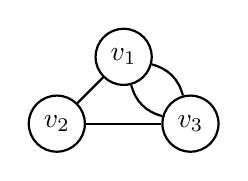
\begin{tikzpicture}[relative, node distance={12mm}, thick, main/.style = {draw, circle}]
    		\node[main] (1) {$v_{1}$};
			\node[main] (2) [below left of=1] {$v_{2}$}; 
			\node[main] (3) [below right of=1] {$v_{3}$}; 
			\draw (1) -- (2);
			\draw (2) -- (3);
			\draw (1) to [out=30, in=150] (3);
			\draw (1) to [out=-30, in=210] (3);
    	\end{tikzpicture}
    \end{center}
    \item \qquad An undirected \textbf{graph} $G$ consists of 2 finite sets: a nonempty set $V$ of \textbf{vertices} and a set E of \textbf{edges}, where each (undirected) edge is associated with a set consisting of either one or two vertices called its \textbf{endpoints}.
    \item \qquad An edge is said to \textbf{connect} its endpoints; two vertices that are connected by an edge are called \textbf{adjacent vertices}; and a vertex that is an endpoint of a loop is said to be \textbf{adjacent to itself}. 
    \item \qquad An edge is said to be \textbf{incident on} each of its endpoints, and two edges incident on the same endpoint are called adjacent edges. We write $e = \{v, w\}$ for an undirected edge $e$ incident on vertices $v$ and $w$.
    \item[Directed Graph] A \textbf{directed graph}, or \textbf{digraph}, $G$, consists of 2 finite sets: a nonempty set $V$ of \textbf{vertices} and a set $E$ of \textbf{directed edges},
where each (directed) edge is associated with an \textbf{ordered pair} of vertices called its \textbf{endpoints}. We write $e = (v, w)$ for a directed edge $e$ from vertex $v$ to vertex $w$.
    \item[\ding{73} Simple Graph] A \textbf{simple graph} is an undirected graph that \textbf{does not} have any loops or parallel edges. (That is, there is at most one edge between each pair of distinct vertices.)
    
    \begin{figure}[H]
		\centering
		\includegraphics[scale=0.4]{simple_graph} 
	\end{figure}
    
    \item[\ding{73} Complete Graph] A \textbf{complete graph} on $n$ \textbf{vertices}, $n > 0$, denoted $\mathbf{K_{n}}$, is a simple graph with $n$ vertices and exactly one edge connecting each pair of distinct vertices. 
    
    \begin{figure}[H]
		\centering
		\includegraphics[scale=0.5]{complete_graph} 
	\end{figure}
	
    \item[\ding{73} Bipartite Graph] A \textbf{bipartite graph} (or bigraph) is a simple graph whose vertices can be divided into two disjoint sets $U$ and $V$ such that every edge connects a vertex in $U$ to one in $V$.
    \item[Complete Bipartite Graph] A complete bipartite graph is a bipartite graph on two disjoint sets $U$ and $V$ such that every vertex in $U$ connects to every vertex in $V$. If $|U|=m$ and $|V|=n$, the complete bipartite graph is denoted as $K_{m, n}$.
    
    \begin{figure}[H]
		\centering
		\begin{tabular}{ll}
			\includegraphics[scale=0.5]{bpt_graph} & \includegraphics[scale=0.5]{complete_bpt_graph} \\
		\end{tabular}
	\end{figure}
    
    \item[Subgraph of a Graph] A graph $H$ is said to be a \textbf{subgraph} of graph $G$ iff every vertex in $H$ is also a vertex in $G$, every edge in $H$ is also an edge in $G$, and every edge in $H$ has the same endpoints as it has in $G$.
    \item[\ding{73} Degree of a Vertex and Total Degree of a Graph] Let $G$ be a graph and $v$ a vertex of $G$. The \textbf{degree} of $v$, denoted $\mathbf{deg(v)}$, equals the number of edges that are incident on $v$, with \textbf{an edge that is a loop counted twice}. The \textbf{total degree of G} is the sum of the degrees of all the vertices of $G$.
    \item[Indegree and outdegree of a Vertex of a Directed Graph] Let $G=(V,E)$ be a directed graph and $v$ a vertex of $G$. The \textbf{indegree} of $v$, denoted $\mathbf{deg}^{-}(\mathbf{v})$ is the number of directed edges that end at $v$. The \textbf{outdegree} of $v$, denoted $\mathbf{deg}^{+}(\mathbf{v})$, is the number of directed edges that originate from $v$.
Note that \[ \sum_{v\;\in\; V} \text{deg}^{-}(v) = \sum_{v\;\in\; V} \text{deg}^{+}(v) = |E| \]
    \item[Walk, Trivial Walk, Trial, Path, Closed Walk] \quad (Let $G$ be a graph, and let $v$ and $w$ be vertices of $G$)
    \item \qquad A \textbf{walk from v to w} is a finite alternating sequence of adjacent vertices and edges of $G$. Thus a walk has the form $v_{0}e_{1}v_{1}e_{2}\dots v_{n-1}e_{n}v_{n}$ where the $v$'s represent vertices, the $e$'s represent edges, $v_{o}=v$, $v_{n}=w$, and for all $i \in \{1,2,\dots,n\}$, $v_{i-1}$ and $v_{i}$ are the endpoints of $e_{i}$. The number of edges, $n$, is the \textbf{length} of the walk.
    \item\qquad The \textbf{trivial walk} from $v$ to $v$ consists of the single vertex $v$.
    \item \qquad A \textbf{trail from v to w} is a walk from $v$ to $w$ that does not contain a repeated edge. 
    \item \qquad A \textbf{path from v to w} is a trail that does not contain a repeated vertex.
    \item \qquad A \textbf{closed walk} is a walk that starts and ends at the same vertex.
    \item[Circuit/Cycle, Simple Circuit/Cycle] \
    \item \qquad A \textbf{circuit} (or \textbf{cycle}) is a closed walk of length at least 3 that does not contain a repeated edge.
    \item \qquad A \textbf{simple circuit} (or \textbf{simple cycle}) is a circuit that does not have any other repeated vertex except the first and last.
    \item \qquad An undirected graph is \textbf{cyclic} if it contains a loop or a cycle; otherwise, it is \textbf{acyclic}.
    \item[Connectedness]\textbf{Two vertices} $v$ and $w$ of a graph $G$ are \textbf{connected} iff there is a \textbf{walk} from $v$ to $w$. \textbf{The graph $G$ is connected} iff given any two vertices $v$ and $w$ in $G$, there is a walk from $v$ to $w$. Symbolically, $G$ is connected iff $\forall$ vertices $v,w\in V(G)$, $\exists$ a walk from $v$ to $w$.
    \item[Connected Component] A graph $H$ is a \textbf{connected component} of a graph $G$ iff 
    \begin{enumerate}
    	\item The graph $H$ is a subgraph of $G$;
		\item The graph $H$ is connected; and
		\item No connected subgraph of $G$ has $H$ as a subgraph and contains vertices or edges that are not in $H$.
    \end{enumerate}
    \item \qquad \emph{(Basically, a subgraph of G that is connected on its own)}
    \item[Euler Circuit and Eulerian Graph] Let $G$ be a graph. An \textbf{Euler circuit} for $G$ is a circuit that contains every vertex and every edge of $G$. An \textbf{Eulerian graph} is a graph that contains an Euler circuit. (See below for examples)
    \begin{figure}[H]
    	\centering
		\includegraphics[scale=0.3]{euler_circuit}
    \end{figure}
    \item[Euler Trail] Let $G$ be a graph, and let $v$ and $w$ be two distinct vertices of $G$. An \textbf{Euler trail/path from} $\mathbf{v}$ \textbf{to} $\mathbf{w}$ is a sequence of adjacent edges and vertices that starts at $v$, ends at $w$, passes through every vertex of $G$ at least once, and traverses every edge of $G$ exactly once.
    \item[Hamiltonian Circuit and Hamiltonian Graph] Given a graph $G$, a \textbf{Hamiltonian circuit} for $G$ is a simple circuit that includes every vertex of $G$. (That is, every vertex appears exactly once, except for the first and the last, which are the same.) A \textbf{Hamiltonian graph} (also called \textbf{Hamilton graph}) is a graph that contains a
Hamiltonian circuit.
	\item[Matrix]An $m\times n$ (read ``m by n'') \textbf{matrix} A over a set $S$ is a rectangular array of elements of $S$ arranged into $m$ rows and $n$ columns. We write $\mathbf{A}=(a_{ij})$.
	\[
	\begin{bmatrix}
		a_{11} & a_{12} & \dots & a_{1j} & \dots & a_{1n} \\
		a_{21} & a_{22} & \dots & a_{2j} & \dots & a_{2n} \\
		\vdots & \vdots &   \   & \vdots &   \   & \vdots \\
		a_{i1} & a_{i2} & \dots & a_{ij} & \dots & a_{in} \\
		\vdots & \vdots &   \   & \vdots &   \   & \vdots \\
		a_{m1} & a_{m2} & \dots & a_{mj} & \dots & a_{mn} \\
	\end{bmatrix}
	\]
	\item \qquad If \textbf{A} and \textbf{B} are matrices, then $\mathbf{A} = \mathbf{B}$ if, and only if, \textbf{A} and \textbf{B} have the same size and the corresponding entries of \textbf{A} and \textbf{B} are all equal; that is, $a_{ij}=b_{ij}$ for all $i=1,2,\dots,m$ and $j=1,2,\dots,n$.
	\item \qquad A matrix for which the numbers of rows and columns are equal is called a \textbf{square matrix}.
	\item \qquad If \textbf{A} is a square matrix of size $n\times n$, then the main diagonal of \textbf{A} consists of all the entries $a_{11},a_{22},\dots,a_{nn}$.
	
    \item[Adjacency Matrix of a Directed Graph] Let $G$ be a directed graph with ordered vertices \iterate{v}{n}. The \textbf{adjacency matrix of} $\mathbf{G}$ is the $n\times n$ matrix $\mathbf{A}=(a_{ij})$ over the set of non-negative integers such that $a_{ij}$ = the number of arrows connecting $v_{i}$ and $v_{j}$ for all $i, j = 1, 2, \dots, n$.
    
		\begin{figure}[H]
			\centering
			\includegraphics[scale=0.5]{adj_matrix}
		\end{figure}
    
    \item[Adjacency Matrix of an Undirected Graph] Let $G$ be an undirected graph with ordered vertices \iterate{v}{n}. The \textbf{adjacency matrix} of $G$ is the $n\times n$ matrix $\mathbf{A}=(a_{ij})$ over the set of non-negative integers such that $a_{ij}$ = the number of edges connecting $v_{i}$ and $v_{j}$ for all $i, j = 1, 2, \dots, n$.
    \item \qquad Note: the adjacency matrix for an undirected graph is symmetric.
    \item[Symmetric Matrix] An $n\times n$ square matrix $A=(a_{ij})$ is called \textbf{symmetric} iff for all $i,j=1,2,\dots, n$, $a_{ij}=a_{ji}$.
    \item[Scalar Product] Suppose that all entries in matrices \textbf{A} and \textbf{B} are real numbers. If the number of elements, $n$, in the $i$th row of \textbf{A} equals the number of elements in the $j$th column of \textbf{B}, then the \textbf{scalar product} or \textbf{dot product} of the $i$th row of A and the $j$th column of \textbf{B} is the real number obtained as follows: 
    \[ 
	\begin{bmatrix}
	   	a_{i1} & a_{i2} & \dots & a_{in} \\
	\end{bmatrix}
	\begin{bmatrix}
    	b_{1j} \\
    	b_{2j} \\
		\vdots \\
		b_{nj} \\
    \end{bmatrix}
    = a_{i1}b_{1j} + a_{i2}b_{2j} + \dots + a_{in}b_{nj}
    \]
    \item[Matrix Multiplication] Let \textbf{A} $= (a_{ij})$ be an $m\times k$ matrix and \textbf{B} $= (b_{ij})$ an $k\times n$ matrix with real entries. The (matrix) product of \textbf{A} times \textbf{B}, denoted \textbf{AB}, is that matrix $(c_{ij})$ defined as
follows:
	\begin{figure}[H]
		\centering
		\includegraphics[scale=0.5]{matrix_multiplication}
	\end{figure}
	\item \qquad where $c_{ij}=a_{i1}b_{1j}+a_{i2}b_{2j}+\dots+a_{ik}b_{kj}=\sum^{k}_{r=1}a_{ir}b_{rj}$ for all $i=1,2,\dots,m$ and $j=1,2,\dots,n$.
	\item \qquad Note: matrix multiplication is \textbf{not commutative} i.e. \textbf{A} $\times$ \textbf{B} $\neq$ \textbf{B} $\times$ \textbf{A} but it is associative, i.e. \textbf{(AB)C} $=$ \textbf{A(BC)}.
	\item[Identity Matrix]For each positive integer $n$, the $n\times n$ \textbf{identity matrix}, denoted $I_{n} = (\delta_{ij})$ or just \textbf{I} (if the size of the matrix is obvious from context), is the $n\times n$ matrix in which all the entries in the main
diagonal are 1’s and all other entries are 0’s. In other words, 
	\[ 
		\delta_{ij}=
		\begin{cases}
			\text{1, if $i=j$} \\
			\text{0, if $i\neq j$} \\
		\end{cases}
	\]
    \item[$\mathbf{n^{th}}$ Power of a Matrix] For any $n \times n$ matrix \textbf{A}, the \textbf{powers of A} are defined as follows: $\mathbf{A^{0}}=\mathbf{I}$ where \textbf{I} is the $n \times n$ identity matrix. $\mathbf{A^{n}}=\mathbf{A\;A^{n-1}}$ for all integers $n\geq 1$.
    \item[Isomorphic Graph] Let $G=(V_{G}, E_{G})$ and $G'=(V_{G'}, E_{G'})$ be two graphs. $G$ is \textbf{isomorphic to} $G'$, denoted $G\cong G'$, if and only if there exist bijections $g:V_{G}\to V_{G'}$ and $h:E_{G}\to E_{G'}$ that preserve the edge-endpoint functions of $G$ and $G'$ in the sense that for all $v\in V_{G}$ and $e\in E_{G}$, $v$ is an endpoint of $e\Leftrightarrow g(v)$ is an endpoint of $h(e)$.
    \item[\ding{73} Alternative definition of Isomorphic Graph] Let $G=(V_{G}, E_{G})$ and $G'=(V_{G'}, E_{G'})$ be two graphs. $G$ is \textbf{isomorphic to} $G'$ if and only if there exists a permutation $\pi:V_{G}\to V_{G'}$ such that $\{u,v\}\in E_{G}\Leftrightarrow \{\pi(u),\pi(v)\}\in E_{G'}$
    
    \begin{figure}[H]
		\centering
		\begin{tabular}{ll}
			\includegraphics[scale=0.6]{isomorphic_graph} &
			\includegraphics[scale=0.6]{isomorphic_bijection}
		\end{tabular}
	\end{figure}
    
    \item[Planar Graph] A \textbf{planar graph} is a graph that can be drawn on a (two-dimensional) plane without edges crossing.
    
    \begin{figure}[H]
		\centering
		\begin{tabular}{ll}
			\includegraphics[scale=0.4]{planar_graph} &
			\includegraphics[scale=0.4]{nonplanar_graph}
		\end{tabular}
	\end{figure}
	
	\item[Kuratowski's Theorem] A finite graph is planar if and only if it does not contain a subgraph that is a subdivision of the complete graph $K_{5}$ or the complete bipartite graph $K_{3,3}$.
    \item[Dominating Set (Tutorial 10 Q9)]A set of vertices, $D$, in an undirected simple graph is said to be a \textbf{dominating set} if every vertex not in $D$ is adjacent to at least one vertex in $D$.
    \item[Minimal Dominating Set (Tutorial 10 Q9)]A \textbf{minimal dominating set} is a dominating set such that none of its proper subsets are dominating sets.
    \item[Complement of a graph (Tutorial 10 Definition 1)]If $G$ is a simple graph, the \emph{complement} of $G$, denoted $\overline{G}$ , is obtained as follows: the vertex set of $\overline{G}$ is identical to the vertex set of $G$. However, two distinct vertices $v$ and $w$ of $\overline{G}$ are connected by an edge if and only if $v$ and $w$ are not connected by an edge in $G$.
    \item[Self-complementary Graph (Tutorial 10 Definition 2)]A \emph{self-complementary graph} is isomorphic with its complement. 
    \item[Triangle (Tutorial 10 Definition 3)]A simple circuit (cycle) of length three is called a \emph{triangle}.
    \item[Proof (Tutorial 10 Q10)]Let $G$ be any any simple graph with 6 vertices. Then $G$ or its complementary graph $\overline{G}$ contains a triangle.

 	% [Ch 12 Trees]
	\vspace{0.2cm}
    \item[\large Trees]\
    \item[Tree] (The graph is assumed to be undirected here.)
    \item \qquad A \textbf{graph} is said to be \textbf{circuit-free} if and only if it has no circuits.
    \item \qquad A graph is called a \textbf{tree} if and only if it is circuit-free and connected.
    \item \qquad A \textbf{trivial tree} is a graph that consists of a single vertex.
    \item \qquad A graph is called a \textbf{forest} if and only if it is circuit-free and not connected.
    
    \begin{figure}[H]
    	\centering
    	\begin{tabular}{lll}
    		\includegraphics[scale=0.5]{graph} & 
    		\includegraphics[scale=0.5]{tree}  &
    		\includegraphics[scale=0.5]{forest} \
    	\end{tabular}
    \end{figure}
    
    \item[Terminal vertex (leaf) and internal vertex]Let $T$ be a tree. If $T$ has only one or two vertices, then each is called a \textbf{terminal vertex} (or \textbf{leaf}). If $T$ has at least three vertices, then a vertex of degree 1 in $T$ is called a \textbf{terminal vertex} (or \textbf{leaf}), and a vertex of degree greater than 1 in $T$ is called an \textbf{internal vertex}.
    \item[Rooted Tree, Level, Height] \
    \item \qquad A \textbf{rooted tree} is a tree in which there is one vertex that is distinguished from the others and is called the \textbf{root}. 
    \item \qquad The \textbf{level} of a vertex is the number of edges along the unique path between it and the root.
    \item \qquad The \textbf{height} of a rooted tree is the maximum level of any vertex of the tree.
    
    \begin{figure}[H]
    	\centering
	    \includegraphics[scale=0.5]{rooted_tree}
	\end{figure}
	
    \item[Child, Parent, Sibling, Ancestor, Descendant] Given the root or any internal vertex $v$ of a rooted tree, the \textbf{children} of $v$ are all those vertices that are adjacent to $v$ and are one level farther away from the root than $v$. If $w$ is a child of $v$, then $v$ is called the \textbf{parent} of $w$, and two distinct vertices that are both children of the same parent are called \textbf{siblings}. Given two distinct vertices $v$ and $w$, if $v$ lies on the unique path between $w$ and the root, then $v$ is an \textbf{ancestor} of $w$, and $w$ is a \textbf{descendant} of $v$.
    \item[Binary Tree / Full Binary Tree]A \textbf{binary tree} is a rooted tree in which every parent has at most two children. Each child is designated either a \textbf{left child} or a \textbf{right child} (but not both), and every parent has at most one left child and one right child. A \textbf{full binary tree} is a binary tree in which \textbf{each parent has exactly two children.}
    
    \begin{figure}[H]
    	\centering
		\includegraphics[scale=0.4]{btree}
    \end{figure}
    
    \item[Left Subtree / Right Subtree]Given any parent $v$ in a binary tree $T$, if $v$ has a left child, then the \textbf{left subtree} of $v$ is the binary tree whose root is the left child of $v$, whose vertices consist of the left child of $v$ and all its descendants, and whose edges consist of all those edges of $T$ that connect the vertices of the left subtree. The \textbf{right subtree} of $v$ is defined analogously.
    \item[Binary Tree Traversal] Tree \textbf{traversal} (also known as \textbf{tree search}) is the process of visiting each node in a tree data structure exactly once in a systematic manner. There are two types of traversal: \textbf{breadth-first search (BFS)} or \textbf{depth-first search (DFS)}. 
    \item \qquad In \textbf{BFS}, it starts at the root and visits its adjacent vertices, and then moves to the next level. 
    \item \qquad In \textbf{DFS}, it starts at the root node and explores as far as possible along each branch before backtracking. 
    \item \qquad There are three types of depth-first traversal: 
	\begin{enumerate}
		\item Pre-order: Current $\to$ Left $\to$ Right
		\item In-order: Left $\to$ Current $\to$ Right 
		\item Post-order: Left $\to$ Right $\to$ Current
	\end{enumerate}
	
	\begin{figure}[H]
		\centering
		\caption{DFS Traversal}
		\includegraphics[scale=0.4]{dfs} \\
		\vspace{0.5cm}
		\caption{BFS Traversal}
		\includegraphics[scale=0.6]{bfs}
	\end{figure}
	
	\item \qquad \hl{Tip: draw 'dots' on the side of the nodes, which represent the order in which they are searched/visited. For pre-order: dot on the left of each node. In-order: dot below node. Post-order: dot to the right of each node.}
	\item \qquad \hl{Tip 2: for pre-order traversal, root is at the start. For post-order, root is at the end. For in-order traversal, root is in the middle of the sequence, and all nodes to the left of the root node are the left children and all nodes to the right of the root node are the right children.}
	\item[Spanning Tree]A \textbf{spanning tree} for a graph $G$ is a subgraph of $G$ that contains every vertex of $G$ and is a tree. 
	\item \qquad (Spanning tree = remove edges from the graph until you cannot remove any more edges without disconnecting the graph)
    \item[Weighted Graph]A \textbf{weighted graph} is a graph for which each edge has an associated positive real number \textbf{weight}. The sum of the weights of all the edges is the \textbf{total weight} of the graph. 
    \item[Minimum Spanning Tree]A \textbf{minimum spanning tree} for a connected weighted graph is a spanning tree that has the least possible total weight compared to all other spanning trees for the graph. If $G$ is a weighted graph and $e$ is an edge of $G$, then $w(e)$ denotes the weight of $e$ and $w(G)$ denotes the total weight of $G$.
    \item[\ding{73} Kruskal's Algorithm for MST] Input: $G$ [a connected weighted graph]
    \begin{enumerate}
    	\item Initialize $T$ to have all the vertices of $G$ and no edges.
		\item Let $E$ be the set of all edges of $G$, and let $m = 0$.
		\item While ($m < n - 1$)
		\begin{enumerate}
			\item Find an edge $e$ in $E$ of least weight.
			\item Delete $e$ from $E$.
			\item If addition of $e$ to the edge set of $T$ does not produce a circuit, then add $e$ to the edge set of $T$ and set $m = m + 1$
		\end{enumerate}
		\item Output: $T$ [$T$ is a minimum spanning tree for $G$]
    \end{enumerate}
    \item[\ding{73} Prim's Algorithm for MST] Input: $G$ [a connected weighted graph with $n$ edges]
    \begin{enumerate}
    	\item Pick a vertex $v$ of $G$ and let $T$ be the graph with this vertex only.
		\item Let $V$ be the set of all vertices of $G$ except $v$.
		\item For $i = 1$ to $n - 1$
		\begin{enumerate}
			\item Find an edge $e$ of $G$ such that (1) $e$ connects $T$ to one of the vertices in $V$, and (2) $e$ has the least weight of all edges connecting $T$ to a vertex in $V$. Let $w$ be the endpoint of $e$ that is in V.
			\item Add $e$ and $w$ to the edge and vertex sets of $T$, and delete $w$ from $V$.
		\end{enumerate}
		\item Output: $T$ [$T$ is a minimum spanning tree for $G$]
    \end{enumerate}
    \item[Djikstra's Algorithm for shortest path] (Not tested AY23/24 Sem1) 
    \begin{enumerate}
    	\item Let $v$ be the \textbf{initial node} (the source). The \textbf{distance} of a node $w$ is defined as the distance from the initial node $v$. 
		\item Set the distances of all nodes to be infinity (except $v$), and mark all nodes as unvisited (including $v$). Set the distance of the initial node to itself as 0. 
		\item Loop: while there are still unvisited nodes, 
		\begin{enumerate}
			\item Pick the vertex with the smallest distance to the initial node $v$ as the \emph{current} node $u$. 
			\item Mark $u$ as visited. 
			\item For \textbf{each} adjacent (neighbouring) node $n$ of the current node that is unvisited, compare the \textbf{current distance} of $n$ with the distance obtained from traversing from $u$ to $n$, i.e. $distance(u) + weight(u, n)$. Take the \textbf{smaller} of the two and set it as the new distance of $n$. 
			\item If there are still unvisited nodes, repeat from step 3. 
		\end{enumerate} 
		\item Return the distance of the target (destination) node from the initial node $v$.
    \end{enumerate}
    \item \hl{Note: there are many variations of Djikstra's Algorithm; some can return you the exact path taken. This version only returns the shortest distance of the target from the source node, but they are all similar in essence.}
    
    
    \newpage
    
    \item[Summary of Definitions] \
	\begingroup
    \setlength{\tabcolsep}{6pt}
	\renewcommand{\arraystretch}{1.75} 
	\begin{table}[H]
		\centering
		\begin{tabular}{|c|p{4in}|}
			\hline 
			Walk & \hfil Can repeat any edges and vertices \\
			\hline
			Trail & \hfil No repeated edges (can revisit vertices) \\
			\hline
			Path & \hfil No repeated edges and no repeated vertices \\ 
			\hline
			Closed Walk & \hfil A walk that starts and ends at the same vertex \\
			\hline
			Circuit & A closed walk of at least length 3 with no repeated edges (can revisit vertices but must end at the start vertex) \\ 
			\hline
			Cycle & Closed walk of at least length 3. No repeated edges, no repeated vertices (except first and last vertex) \\
			\hline
			Cyclic & \hfil Any graph that contains a cycle or a loop \\
			\hline
			Acyclic & \hfil Not cyclic (no cycle or loop) \\
			\hline
			Connected vertices & \hfil There is a walk from $v$ to $w$ \\
			\hline
			Connected graph & \hfil Given \emph{any} two vertices, there is a walk between them \\
			\hline
			Euler Circuit & Circuit containing every vertex and traversing every edge only once. I.e. no repeated edges, but you can revisit vertices. You must start and end at the same vertex \\
			\hline
			Euler Graph & \hfil Contains an Euler Circuit \\
			\hline
			Euler Trail & Start at $v$, end at $w$, contains every vertex of $G$ (can revisit vertices) and traverses every edge exactly once \\
			\hline
			Hamiltonian Circuit & Visit every vertex exactly once (except first and last vertex, must start and end at same vertex). Inherently, there won't be any repeated edges  \\
			\hline 
			Hamiltonian Graph & \hfil Contains a Hamiltonain Circuit \\ 
			\hline
			Hamiltonian Trail & \hfil Start at $v$, end at $w$, must visit every vertex in $G$ exactly once \\
			\hline
			Simple Graph & \hfil No loops (to self) and no parallel edges \\
			\hline
			Complete Graph & Simple graph with exactly one edge between each pair of distinct vertices. Denoted $K_{n}$ where $n$ is the number of vertices \\ 
			\hline
			Bipartite Graph & Vertex set split into two disjoint sets such that vertices in one set only has edges to vertices in the other set \\
			\hline
			Tree & \hfil Connected and circuit-free graph \\ 
			\hline 
			Trivial Tree & \hfil Graph with only one vertex \\
			\hline 
			Forest & \hfil Not connected but circuit-free graph \\
			\hline
			Spanning Tree & \hfil Contains every vertex of $G$ and is a tree \\ 
			\hline
			MST & \hfil Spanning tree with the least possible weight \\
			\hline
		\end{tabular}
	\end{table}	  
	\endgroup
	
	\item \emph{Note: Epp and CS1231S refer to a `cycle' as a `simple circuit'. Euler Trails are loosely referred to as Euler Paths but they are NOT paths because you can still repeat vertices.}
	
\end{description}

% ================================ THEOREMS AND LEMMAS ===================================

\newpage
\section*{Theorems, Lemmas \& Corollaries}
\hrule
\vspace{0.3cm}
\begin{description}

	% 2 - Compound Statements 
    \item[Theorem 2.1.1 Logical Equivalences]Given any statement variables $p$, $q$ and $r$, a tautology is \textbf{true} and a contradiction is \textbf{false}: 
    \begin{table}[h]
        \centering
        {\rowcolors{1}{white}{lightgray!20}
        \begin{tabular}{|c|c|c|c|}
            \hline
             1 & Commutative Laws & $p \wedge q\equiv q\wedge p$ & $p \vee q\equiv q\vee p$ \\
             2 & Associative Laws & $p\wedge q\wedge r\equiv (p\wedge q)\wedge r\equiv p\wedge(q\wedge r)$ & $p\vee q\vee r\equiv (p\vee q)\vee r\equiv p\vee(q\vee r)$ \\
             3 & Distributive Laws & $p\wedge (q\vee r)\equiv(p\wedge q)\vee(p\wedge r)$ & $p\vee (q\wedge r)\equiv(p\vee q)\wedge(p\vee r)$ \\ 
             4 & Identity Laws & $p\wedge\text{\textbf{true}}\equiv p$ & $p\vee\text{\textbf{false}}\equiv p$ \\
             5 & Negation Laws & $p\vee{\sim} p\equiv\text{\textbf{true}}$ & $p\wedge{\sim} p\equiv\text{\textbf{false}}$ \\
             6 & Double Negation Law & ${\sim}({\sim} p)\equiv p$ &  \\
             7 & Idempotent laws & $p\wedge p\equiv p$ & $p\vee p\equiv p$ \\
             8 & Universal bound laws & $p\vee\text{\textbf{true}}\equiv\text{\textbf{true}}$ & $p\wedge\text{\textbf{false}}\equiv\text{\textbf{false}}$ \\
             9 & De Morgan's laws & ${\sim}(p\wedge q)\equiv{\sim} p\vee{\sim} q$ & ${\sim}(p\vee q)\equiv{\sim} p\wedge{\sim} q$ \\
             10 & Absorption laws & $p\vee(p\wedge q)\equiv p$ & $p\wedge(p\vee q)\equiv p$ \\
             11 & Negation of \textbf{true} and \textbf{false} & ${\sim}\text{\textbf{true}}\equiv\text{\textbf{false}}$ & ${\sim}\text{\textbf{false}}\equiv\text{\textbf{true}}$ \\
            \hline
        \end{tabular}}
        \label{tab:1}
    \end{table}
    \item[Implication Law]$p\to q\equiv {\sim} p\vee q $ 
    \item[Table 2.3.1 Rules of Inference] (Quote the rules if you use them in proofs)
    \begin{table}[h]
    	\centering
		{\rowcolors{1}{white}{lightgray!20}
		\begin{tabular}{|c|c|c|c|} 
			\hline
			Rule of Inference & & Rule of Inference & \\
			\hline
			Modus Ponens & $p\to q$ \quad $p$ \quad $\bullet$q & Elimination & $p\lor q$ \quad ${\sim} q$ \quad $\bullet p$ \\
			Modus Tollens & $p\to q$ \quad ${\sim} q$ \quad $\bullet{\sim} p$ & Transitivity & $p\to q$ \quad $q\to r$ \quad $\bullet p\to r$ \\
			Generalization &  $p$ \quad $\bullet p\lor q$ & Proof by Division into Cases  & $p\lor q$ \quad $p\to r$ \quad $q\to r$ \quad $\bullet r$ \\
			Specialization &  $p\land q$ \quad $\bullet p$ & Contradiction Rule & ${\sim}{p}\to\text{\textbf{false}}$ \quad $\bullet p$ \\
			Conjuction & $p$ \quad $q$ \quad $\bullet p\land q$ & \ & \\
			\hline
		\end{tabular}}
		\label{tab:2}
    \end{table}
    
	% 3 - Quantified Statements
    \item[Theorem 3.2.1 Negation of Universal Statement] The \textbf{negation} of a statement of the form $\forall x\in D, P(x)$ is logically equivalent to a statement of the form $\exists x\in D$ such that ${\sim} P(x)$. Symbolically, ${\sim}(\forall x\in D, P(x)) \equiv \exists x\in D \text{ such that } {\sim} P(x)$.
    \item[Theorem 3.2.2 Negation of an Existential Statement] The \textbf{negation} of a statement of the form $\exists x\in D, P(x)$ is logically equivalent to a statement of the form $\forall x\in D$ such that ${\sim} P(x)$. Symbolically, ${\sim}(\exists x\in D, P(x)) \equiv \forall x\in D \text{ such that } {\sim} P(x)$.
    \item[Rules of Inference (Quantified Statements)] \
    \begin{table}[h]
        \centering
        {\rowcolors{1}{white}{lightgray!20}
        \begin{tabular}{|c|c|}
            \hline
             Rule of Inference & Name \\
             \hline
             $\forall x\in D P(x)$ \quad $\therefore P(a)$ if $a\in D$ & Universal instantiation \\
             $P(a)$ for every $a\in D$ \quad $\therefore \forall x\in D P(x)$ & Universal generalization \\
             $\exists x\in D P(x)$ \quad $\therefore P(a)$ for some $a\in D$ & Existential instantiation \\
             $P(a)$ for some $a\in D$ \quad  $\therefore \exists x\in D P(x)$ & 	Existential generalization \\
            \hline
        \end{tabular}}
        \label{tab:1}
    \end{table}

	% 4 - Methods of Proofs 
    \item[Theorem 4.2.1 (5th: 4.3.1)] Every integer is a rational number.
    \item[Theorem 4.2.2 (5th: 4.3.2)] The sum of any two rational numbers is rational.
    \item[Corollary 4.2.3 (5th: 4.2.3)] The double of a rational number is rational.
    \item[Theorem 4.3.1 (5th: 4.4.1) A Positive Divisor of a Positive Integer:] For all positive integers $a$ and $b$, if $a|b$, then $a\leq b$. 
    \item[Theorem 4.3.2 (5th: 4.4.2) Divisors of 1:] The only divisors of 1 are 1 and -1.
    \item[Theorem 4.3.3 (5th: 4.4.3) Transitivity of Divisibility:] For all integers $a$, $b$ and $c$, if $a|b$ and $b|c$, then $a|c$. 
    \item[Theorem 4.4.1 The Quotient-Remainder Theorem]Given any integer $n$ and a positive integer $d$, there exists unique integers $q$ and $r$ such that $n=dq+r$ and $0\leq r < d$.
    \item[Theorem 4.6.1 (5th: 4.7.1)] There is no greatest integer.
    \item[Theorem 4.6.4 (5th: 4.7.4)] For all integers $n$, if $n^{2}$ is even then $n$ is even.
    \item[Proof (Tutorial 1 Q10)] The product of any two odd integers is an odd integer.
    \item[Proof (Tutorial 1 Q11)] $n^{2}$ is odd if and only if $n$ is odd.
    \item[Proof (Tutorial 2 Q4(a))]Integers are not closed under division.
    \item[Proof (Tutorial 2 Q4(b))]Rational numbers are closed under addition.
    \item[Proof (Tutorial 2 Q4(c))]Rational numbers are not closed under division.
    \item[Proof (Tutorial 2 Q8)]$\forall x\in \mathbb{R} ((x^{2}>x)\to (x<0)\lor(x>1))$.
    \item[Proof (Tutorial 2 Q11)]If $n$ is a product of two positive integers $a$ and $b$, then $a\leq n^{1/2}$ or $b\leq n^{1/2}$.
    \item[Theorem 4.7.1 (5th: 4.8.1)] $\sqrt{2}$ is irrational.
    
    \item[Theorem 5.1.1] If $a_{m}, a_{m+1},a_{m+2},\dots$ and $b_{m}, b_{m+1},b_{m+2},\dots$ are sequences of real numbers and $c$ is any real number, then the following equations hold for any integer $n\geq m$: 
    \begin{flalign*}
    &1.\quad \sum_{k=m}^{n}a_{k} + \sum_{k=m}^{n}b_{k} = \sum_{k=m}^{n}(a_{k}+b_{k}) &\\
    &2.\quad c\cdot\sum_{k=m}^{n}a_{k}=\sum_{k=m}^{n}c\cdot a_{k} &\\
    &3.\quad (\prod_{k=m}^{n}a_{k})\cdot(\prod_{k=m}^{n}b_{k})=(\prod_{k=m}^{n}(a_{k}\cdot b_{k})) &\\
    \end{flalign*}
    \item[Theorem 5.2.2 (5th: 5.2.1) Sum of first $n$ Integers] For all integers $n\geq 1$, $1+2+3+...+n=\frac{n(n+1)}{2}$.
    \item[Theorem 5.2.3 (5th: 5.2.2) Sum of a Geometric Sequence] For any real number $r\neq 1$, and any integers $n\geq 0$, \[\sum_{i=0}^{n}r^{i}=\frac{r^{n+1}-1}{r-1}\]
    \item[Proposition 5.3.1 (5th: 5.3.2)] For all integers $n\geq 0$, $2^{2n}-1$ is divisible by 3.  
    \item[Proposition 5.3.2 (5th: 5.3.3)] For all integers $n\geq 3$, $2n+1<2^{n}$.
    \item[Proof (Lecture 8 Slide 39)] For $n\in\mathbb{Z}^{+}$, any $2^{n}\times 2^{n}$ board with one square removed can be tiled by L-trominoes. 
    \item[Proof (Lecture 8 Slide 45)] Any integer $>$ 1 is divisible by a prime number.
    
    % 5 - Sets
    \item[Theorem 6.2.1 Subset Relations] \
    \begin{description}
    	\item[1. Inclusion of Intersection:] For all sets $A$ and $B$, (a) $A\cap B\subseteq A$ \qquad (b) $A\cap B \subseteq B$.
		\item[2. Inclusion in Union:] For all sets $A$ and $B$, (a) $A\subseteq A\cup B$ \qquad (b) $B\subseteq A\cup B$.
		\item[3. Transitive Property Of Subsets:] For all sets $A$, $B$ and $C$, $A\subseteq B\land B\subseteq C\to A\subseteq C$.
    \end{description}
	\item[Theorem 6.2.2 Set Identities] Let all sets referred to below be subsets of a universal set $U$. 

    \begin{table}[H]
        \centering
        {\rowcolors{1}{white}{lightgray!20}
        \begin{tabular}{|c|c|c|c|}
            \hline
             1 & Commutative Laws & $A \cup B = B\cup A$ & $A \cap B=B\cap A$ \\
             2 & Associative Laws & $(A\cup B)\cup C=A\cup(B\cup C)$ & $(A\cap B)\cap C=A\cap(B\cap C)$ \\
             3 & Distributive Laws & $A\cup (B\cap C)=(A\cup B) \cap (A\cup C)$ & $A\cap (B\cup C)=(A\cap B)\cup (A\cap C)$ \\ 
             4 & Identity Laws & $A\cup\emptyset = A$ & $A\cap U=A$ \\
             5 & Complement Laws & $A\cup \overline{\rm A}=U$ & $A\cap \overline{A} = \emptyset$ \\
             6 & Double Complement Law & $\overline{\overline{A}} = A$ &  \\
             7 & Idempotent Laws & $A\cup A = A$ & $A\cap A = A$ \\
             8 & Universal Bound Laws & $A\cup U=U$ & $A\cap \emptyset = \emptyset$ \\
             9 & De Morgan's Laws & $\overline{A\cup B} = \overline{A} \cap \overline{B}$ & $\overline{A\cap B} = \overline{A} \cup \overline{B}$ \\
             10 & Absorption Laws & $A\cup (A\cap B)=A$ & $A\cap(A\cup B)=A$ \\
             11 & Complements of $U$ and $\emptyset$ & $\overline{U} = \emptyset$ & $\overline{\emptyset} = U$ \\
             12 & Set Difference Law & $A\setminus B=A\cap \overline{B}$ & \\
            \hline
        \end{tabular}}
        \label{tab:1}
    \end{table}

    \item[Theorem 6.2.4] An empty set is a \textbf{subset} of every set, i.e. $\emptyset\subseteq A$ for all sets $A$.
    \item Note: a set with exactly one element is called a \textbf{singleton}.
    \item[Theorem: Cardinality of a Power Set of a Finite Set]Let $A$ be a finite set where $|A|=n$, then $|P(A)|=2^{n}$. 
    \item[Theorem 6.3.1] Suppose A is a finite set with $n$ elements, then $P(A)$ has $2^{n}$ elements. In other words, $|P(A)|=2^{|A|}$.
    
	 % 6 - Relations
	 \item[Theorem 8.3.1 Relation Induced by a Partition]Let $A$ be a set with a partition and let $R$ be the relation induced by the partition. Then $R$ is reflexive, symmetric, and transitive.
	 \item[Lemma Rel.1 Equivalence Classes]Let $\sim$ be an equivalence relation on a set $A$. The following are equivalent for all $x, y\in A$. (i)$x\sim y$ \qquad (ii) $[x]=[y]$ \qquad (iii) $[x]\cap[y]\neq \emptyset$.
	 \item[Theorem 8.3.4 The Partition Induced by an Equivalence Relation] If $A$ is a set and $R$ is an equivalence relation on $A$, then the distinct equivalence classes of $R$ form a partition of $A$; that is, the union of the equivalence classes is all of $A$, and the intersection of any two distinct classes is empty.
	 \item[Theorem Rel.2 Equivalence classes form a partition]Let $\sim$ be an equivalence relation on a set $A$. Then $A/{\sim}$ is a partition of $A$.
	 
	 % 7 - Functions
	 \item[Theorem 7.1.1 Function Equality]Two functions $f:A\to B$ and $g:C\to D$ are equal, i.e. $f=g$, iff (i)$A=C$, and (ii) $f(x)=g(x)\;\forall x\in A$.
	 \item[Theorem 7.2.3] If $f:X\to Y$ is a bijection, then $f^{-1}:Y\to X$ is also a bijection. In other words, $f:X\to Y$ is bijective iff $f$ has an inverse.
	 \item[Theorem 7.3.1 Composition with an Identity Function]If $f$ is a function from set $X$ to set $Y$, and $id_{x}$ is the identity function on $X$, and $id_{y}$ is the identity function on $Y$, then $f\circ id_{x}=f$ and $id_{y}\circ f=f$.
	 \item[Theorem 7.3.2 Composition of a Function with its Inverse]If $f:X\to Y$ is a bijection with the inverse function $f^{-1}:Y\to X$, then $f^{-1}\circ f=id_{x}$ and $f\circ f^{-1}=id_{y}$.
	 \item[Theorem: Associativity of Function Composition]Let $f:A\to B$, $g:B\to C$ and $h:C\to D$. Then $(h\circ g)\circ f = h\circ (g\circ f)$. Function composition is associative. 
	 \item[Theorem 7.3.3] If $f:X\to Y$ and $g:Y\to Z$ are both injective, then $g\circ f$ is injective. 
	 \item[Theorem 7.3.4] If $f:X\to Y$ and $g:Y\to Z$ are both surjective, then $g\circ f$ is surjective.
	 \item[Theorem: Equality of Cardinality of Finite Sets]Let $A$ and $B$ be any finite sets.
 iff there is a bijection $f:A\to B$.
	\item[Theorem 7.4.1 Properties of Cardinality]The same-cardinality relation is an equivalence relation. For all sets $A$, $B$ and $C$: 
	\item \qquad \textbf{Reflexive}: $|A|=|A|$
	\item \qquad \textbf{Symmetric}: $|A|=|B|\to|B|=|A|$
	\item \qquad \textbf{Transitive}: $(|A|=|B|)\land(|B|=|C|)\to|A|=|C|$.
	\item[Theorem: $\mathbb{Z}^{+} \times \mathbb{Z}^{+}$ is countable] \
	\item[Theorem (Cartesian Product)]If sets $A$ and $B$ are both countably infinite, then so is $A \times B$.
	\item[Corollary (General Cartesian Product)]Given $n\geq 2$ countably infinite sets $A_{1}, A_{2}, \dots, A_{n}$ the Cartesian product $A_{1} \times A_{2} \times \dots \times A_{n}$ is also countably infinite.
	\item[Theorem: Unions (Lecture 9 Slide 30)]The union of countably many countable sets is countable. That is, if $A_{1}, A_{2}, \dots$ are all countable sets, then so is \[\bigcup_{i=1}^{\infty}A_{i}\]
	\item[Proposition 9.1]An infinite set $B$ is countable if and only if there is a sequence $b_{0}, b_{1}, b_{2} \dots \in B$ in which every element of $B$ appears exactly once. 
	\item \qquad (Definition of sequence) A \textbf{sequence} $a_{0}, a_{1}, a_{2}, \dots$ can be represented by a function $a$ whose domain is $\mathbb{Z}_{\geq0}$ that satisfies $a(n)=a_{n}$ for every $n\in\mathbb{Z}_{\geq0}$.
	\item[Lemma 9.2 Countability via Sequence]An infinite set $B$ is countable if and only if there is a sequence $b_{0}, b_{1}, b_{2} \dots$ in which every element of $B$ appears.
	\item[Theorem 7.4.2 (Cantor)] The set of real numbers between 0 and 1, $(0,1)=\{x\in\mathbb{R}\;|\;0<x<1\}$, is uncountable. To prove that a a set is uncountable means proving that there is no possibility of a bijection from that set to $\mathbb{Z}^{+}$.
	\item[Theorem 7.4.3]Any subset of any countable set is countable.
	\item[Corollary 7.4.4 (Contrapositive of Theorem 7.4.3)]Any set with an uncountable subset is uncountable.
	\item \qquad Corollary 7.4.4 implies that $\mathbb{R}$ is uncountable since $(0,1)\subseteq\mathbb{R}$ and $(0,1)$ is uncountable.
	\item[Proposition 9.3]Every infinite set has a countably infinite subset.
	\item[Lemma 9.4 Union of Countably Infinite Sets]Let $A$ and $B$ be countably infinite sets. Then $A\cup B$ is countable.
	\item[Theorem 9.1.1 The Number of Elements in a List] If $m$ and $n$ are integers and $m\leq n$, then there are $n-m+1$ integers from $m$ to $n$ inclusive.
	\item[Theorem 9.2.1 The Multiplication/Product Rule]If an operation consists of $k$ steps and the first step can be performed in $n_{1}$ ways, the second step can be performed in $n_{2}$ ways (regardless of how the first step was performed), the $k^{th}$ step can be performed in $n_{k}$ ways, (regardless of how the preceding steps were performed), then the entire operation can be performed in $n_{1}\times n_{2} \times n_{3} \times \dots n_{k}$ ways.
	\item[Theorem 9.2.2 Permutations]The number of permutations of a set with $n$ ($n\geq 1$) elements is $n!$.
	\item[Theorem 9.2.3 r-permutations from a set of $n$ elements]If $n$ and $r$ are integers and $1\leq r\leq n$, then the number of r-permutations of a set of $n$ elements is given by the formula $P(n, r) = n(n – 1)(n – 2) \dots (n – r + 1)$. Or equivalently, $P(n,r)=\frac{n!}{(n-r)!}$.
	\item[Theorem 9.3.1 The Addition/Sum Rule]Suppose a finite set $A$ equals the union of $k$
distinct mutually disjoint subsets $A_{1}, A_{2}, \dots, A_{k}$. Then $|A|=|A_{1}|+|A_{2}|+\dots+|A_{k}|$.
	\item[Theorem 9.3.2 The Difference Rule] If $A$ is a finite set and $B\subseteq A$, then $|A\setminus B|=|A|-|B|$.
	\item \qquad How it's derived: If $B\subseteq A$, then the two sets $B$ and $A\setminus B$ have no elements in common and $B\cup (A\setminus B) = A$. Hence, by addition rule, $|B|+|A\setminus B|=|A|$. Subtracting $|B|$ from both sides gives the equation $|A\setminus B|=|A|-|B|$.
	\item[Theorem 9.3.3 The Inclusion/Exclusion Rule for 2 or 3 Sets] If $A$, $B$, and $C$ are any finite sets, then $|A\cup B|=|A|+|B|-|A\cap B|$ and $|A\cup B\cup C| = |A| + |B| + |C| - |A\cap B| - |A\cap C| - |B\cap C| + |A\cap B\cap C|$.
	\item[Theorem 9.5.1 Formula for ${n\choose r}$]The number of subsets of size $r$ (or r-combinations) that can be chosen from a set of $n$ elements, ${n\choose r}$, is given by the formula ${n\choose r} = \frac{P(n,r)}{r!}$\; or equivalently, ${n\choose r}=\frac{n!}{r!(n-r)!}$ where $n$ and $r$ are non-negative integers with $r\leq n$.
	\item[Theorem 9.5.2 Permutations with sets of indistinguishable objects]Suppose a collection consists of $n$ objects of which $n_{1}$ are of type 1 and are indistinguishable from each other, $n_{2}$ are of type 2 and are indistinguishable from each other,$\dots$ $n_{k}$ are of type k and are indistinguishable from each other, and suppose that $n_{1}+n_{2}+\dots+n_{k}=n$. Then the number of distinguishable permutations of the $n$ objects is \[{n\choose r}{n-n_{1}\choose n_{2}}{n-n_{1}-n_{2}\choose n_{3}}\dots{n-n_{1}-n_{2}-\dots-n_{k-1}\choose n_{k}} = \frac{n!}{n_{1}!n_{2}!n_{3}!\dots n_{k}!} \]
	\item[Theorem 9.6.1 Number of r-combinations with Repetition Allowed]The number of r-combination with repetition allowed (multisets of size $r$) that can be selected from a set of $n$ elements is: $r+n-1\choose r$. This equals the number of ways $r$ objects can be selected from $n$ categories of objects with repetitions allowed.
	\item[Formula to Use] \
	\begingroup
	\setlength{\tabcolsep}{6pt} % Default value: 6pt
	\renewcommand{\arraystretch}{1.75} % Default value: 1
	\begin{table}[H]
		\centering
		\begin{tabular}{|c|c|c|}
			\hline
			& \textbf{Order Matters} & \textbf{Order Does Not Matter} \\
			\hline
			\textbf{Repetition Is Allowed} & $n^{k}$ & ${k+n-1 \choose k}$ \\
			\hline
			\textbf{Repetition Is Not Allowed} & $P(n, k)$ & ${n\choose k}$\\
			\hline
		\end{tabular}
	\end{table}	     
	\endgroup
	
	\item[Theorem 9.7.1 Pascal’s Formula]Let $n$ and $r$ be positive integers, $r\leq n$. Then ${n+1\choose r}={n\choose r-1}+{n\choose r}$. 
	\item[Theorem 9.7.2 Binomial Theorem] Given any real numbers $a$ and $b$ and any non-negative integer $n$, \[(a+b)^{n}=\sum_{k=0}^{n}{n\choose k}a^{n-k}b^{k}=a^{n}+{n\choose 1}a^{n-1}b^{1} + {n\choose 2}a^{n-2}b^{2}+\dots+{n\choose n-1}a^{1}b^{n-1} + b^{n} \]
	\item[Theorem 9.9.1 Bayes’ Theorem]Suppose that a sample space $S$ is a union of mutually disjoint events $B_{1}, B_{2}, B_{3},\dots,B_{n}$. Suppose $A$ is an event in $S$, and suppose $A$ and all the $B_{i}$ have non-zero probabilities. If $k$ is an integer with $1\leq k\leq n$, then \[ P(B_{k}|A) = \frac{P(A|B_{k})\cdot P(B_{k})} {P(A|B_{1})\cdot P(B_{1})+P(A|B_{2})\cdot P(B_{2})+\dots+P(A|B_{n})\cdot P(B_{n}) } \]
	
	\item[Theorem 10.1.1 The Handshake Theorem] If the vertices of $G$ are \iterate{v}{n}, where $n\geq 0$, then the total degree of $G$ = $deg(v_{1}) + deg(v_{2}) + \dots + deg(v_{n}) = 2 \times \text{the number of edges of } G$.
	\item[Proof (Tutorial 11 Discussion Q1)] For a simple connected graph with $n$ $(n>0)$ vertices, there are minimum $(n - 1)$ edges and maximum $\frac{n(n-1)}{2}$ edges.
	\item \qquad (Since the graph is connected, there is a unique path from every vertex to every other vertex, and removing any edge will make the graph disconnected. Thus the minimum number of edges is $n-1$. Max number of edges can be derived from Handshake Theorem, which is the sum of the AP series $1 + 2 + \dots + (n-1)$.)
	\item[Proof (Tutorial 11 Discussion Q2)] For a graph with $n$ $ (n > 1)$ vertices, there are $2^{n \choose 2}$ simple graphs. 
	\item \qquad This is because there are maximum $\frac{n(n-1)}{2}$ edges which is equivalent to $n\choose 2$. For each edge, you can either include or not include it, hence the number of permutations is 2 to the power of the maximum number of edges.
	\item[Corollary 10.1.2] The total degree of a graph is even.
	\item[Proposition 10.1.3]In any graph there are an even number of vertices of odd degree.
	\item[\ding{73} Lemma 10.2.1]Let G be a graph.
	\item \qquad a. If $G$ is connected, then any two distinct vertices of $G$ can be connected by a path.
	\item \qquad b. If vertices $v$ and $w$ are part of a circuit in $G$ and one edge is removed from the circuit, then there still exists a trail from $v$ to $w$ in $G$.
	\item \qquad c. If $G$ is connected and $G$ contains a circuit, then an edge of the circuit can be removed without disconnecting $G$.
	\item[Proof (Tutorial 11 Q5)] Let $G=(V,E)$ be a simple, undirected graph. If $G$ is connected, then $|E|\geq|V|-1$.
	\item[Proof (Tutorial 11 Q6)] Let $G=(V,E)$ be a simple, undirected graph. If $G$ is acyclic, then $|E|\leq|V|-1$.
	\item[Theorem 10.2.2]If a graph has an Euler circuit, then every vertex of the graph has positive even degree.
	\item[Contrapositive Version of Theorem 10.2.2]If some vertex of a graph has odd degree, then the graph doesn’t have an Euler circuit.
	\item[Theorem 10.2.3]If a graph $G$ is \emph{connected} and the degree of every vertex of G is a positive \emph{even integer}, then $G$ has an Euler circuit.
	\item[Theorem 10.2.4]A graph $G$ has an Euler circuit iff $G$ is connected and every vertex of $G$ has positive even degree.
	\item[Corollary 10.2.5] Let $G$ be a graph, and let $v$ and $w$ be two distinct vertices of $G$. There is an Euler trail from $v$ to $w$ iff $G$ is connected, $v$ and $w$ have odd degree, and all other vertices of $G$ have positive even degree.
	\item[Proposition 10.2.6]If a graph $G$ has a Hamiltonian circuit, then $G$ has a subgraph $H$ with the following properties:
	\begin{enumerate}
		\item $H$ contains every vertex of $G$.
		\item $H$ is connected.
		\item $H$ has the same number of edges as vertices.
		\item Every vertex of $H$ has degree 2.
	\end{enumerate}
	\item[Theorem 10.3.2] If $G$ is a graph with vertices $v_{1}, v_{2}, \dots, v_{m}$ and \textbf{A} is the adjacency matrix of $G$, then for each positive integer $n$ and for all integers $i, j = 1, 2, \dots, m$, the $ij$-th entry of $\mathbf{A}^{n}$ = the number of walks of length $n$ from $v_{i}$ to $v_{j}$.
	\item \qquad (Note: $\mathbf{A^{0}}$ is the identity matrix \textbf{I}. See definitions for $n^{th}$ power of a matrix.)
	\item[Theorem 10.4.1 Graph Isomorphism is an Equivalence Relation]Let $S$ be a set of graphs and let $\cong$ be the relation of graph isomorphism on $S$. Then $\cong$ is an equivalence relation on $S$.
	\item[Euler's Formula]For a connected planar simple graph $G = (V, E)$ with $e = |E|$ and $v = |V|$, if we let $f$ be the number of faces, then $f = e - v + 2$.
	
	\begin{figure}[H]
		\centering
		\includegraphics[scale=0.4]{eulers_formula}
	\end{figure}
	\item[Proof (Tutorial 11 Q2)] For any planar graph with $f$ faces, $v$ vertices and $e$ edges, (a) $3f\leq 2e$, and (b) $e\leq 3v-6$.
	\item \qquad (a) This is because each face must have at least 3 edges, and each each can be counted at most 2 times (borders between 2 faces), so there is an upper bound of $2e$.
	\item \qquad (b) Derived from Euler's formula, or just by counting the number of edges.
	
	\item[Lemma 10.5.1]Any non-trivial tree has at least one vertex of degree 1.
	\item[\ding{73} Theorem 10.5.2]Any tree with $n$ vertices ($n > 0$) has $n-1$ edges.
	\item[\ding{73} Lemma 10.5.3]If $G$ is any connected graph, $C$ is any circuit in $G$, and one of the edges of $C$ is removed from $G$, then the graph that remains is still connected.
	\item[\ding{73} Theorem 10.5.4]If $G$ is a connected graph with $n$ vertices and $n-1$ edges, then $G$ is a tree.
	\item[Proof (Tutorial 11 Q7)] Let $G=(V,E)$ be a simple, undirected graph. $G$ is a tree iff there is exactly one path between every pair of vertices. 
	\item[\ding{73} Lemma 10.5.5] Let $G$ be a simple, undirected graph. Then if there are two distinct paths from a vertex $v$ to a different vertex $w$, then $G$ contains a cycle (and hence $G$ is cyclic).
	\item \qquad (i.e. 2 distinct paths from $v$ to $w$ $\Rightarrow$ G is cyclic \quad $||$  \quad G is acyclic $\Rightarrow$ at most one distinct path from $v$ to $w$ (contrapositive))
	\item[Theorem 10.6.1 Full Binary Tree Theorem]If $T$ is a full binary tree with $k$ internal vertices, then $T$ has a total of $2k + 1$ vertices and has $k + 1$ terminal vertices (leaves).
	\item[Theorem 10.6.2]For non-negative integers $h$, if $T$ is any binary tree with height $h$ and $t$ terminal vertices (leaves), then $t\leq 2^{h}$. Equivalently, $log_{2}t\leq h$.
	\item[Proposition 10.7.1] \
	\item \qquad 1. Every connected graph has a spanning tree.
	\item \qquad 2. Any two spanning trees for a graph have the same number of edges.

\end{description}

% ====================================== PROOFS =======================================
	 
\newpage
\begingroup

% set new style
\renewcommand{\labelenumii}{\arabic{enumi}.\arabic{enumii}}
\renewcommand{\labelenumiii}{\arabic{enumi}.\arabic{enumii}.\arabic{enumiii}}
\renewcommand{\labelenumiv}{\arabic{enumi}.\arabic{enumii}.\arabic{enumiii}.\arabic{enumiv}}

\section*{Examples of Proofs (For reference)}
\hrule
\vspace{0.5cm}

% Format for Proofs
%\begin{enumerate}
%	\item Item 1 
%	\item Item 2 
%	\begin{enumerate}
%		\item Sub-item 1
%	\end{enumerate}
%	\item Item 3
%	\item Conclusion
%\end{enumerate}

% If on Mac, use Command + Shift + [ or ] to comment/uncomment multiple lines together

\subsection*{Prove that the product of two consecutive odd numbers is always odd.}
\begin{enumerate}
    \item Let $a$ and $b$ be the two consecutive odd numbers. 
    \begin{enumerate}
        \item WLOG, assume that $a<b$, hence $b=a+2$.
        \item Now, $a=2k+1$ for some integer $k$ (by definition of odd numbers).
        \item Similarly, $b=a+2=2k+3$.
        \item Therefore, $ab=(2k+1)(2k+3)=(4k^2+6k)+(2k+3)=4k^2+8k+3=2(2k^2+4k+1)+1$ (by basic algebra).
        \item Let $m=(2k^2+4k+1)$, which is an integer (by closure of integers under $\times$ and +. 
        \item Then $ab=2m+1$, which is odd (by definition of odd numbers).
    \end{enumerate}
    \item Therefore, the product of two consecutive odd numbers is always odd.
\end{enumerate}
\vspace{0.1cm}

\subsection*{Prove that the following statement is false: The product of two irrational numbers is always irrational.}
\begin{enumerate}
    \item Let them two irrational numbers be $\sqrt{2}$ and $\sqrt{8}$. 
    \begin{enumerate}
        \item Then $\sqrt{2}\times\sqrt{8}=\sqrt{16}=4$, which is a rational number (by basic algebra).
    \end{enumerate}
    \item Therefore, the statement ``the product of two irrational numbers is always irrational'' is false.
\end{enumerate}
\paragraph{Note:}One counter-example is sufficient. 
\vspace{0.1cm}

\subsection*{Prove that the difference of two consecutive squares between 30 and 100 is odd. (Proof by exhaustion / brute force)}
\begin{enumerate}
    \item The squares between 30 and 100 are 36, 49, 64 and 81.
    \begin{enumerate}
        \item Case 1: 49 – 36 = 13 which is odd.
        \item Case 2: 64 – 49 = 15 which is odd.
        \item Case 3: 81 – 64 = 17 which is odd.
    \end{enumerate}
    \item Therefore, the difference of two consecutive squares
between 30 and 100 is odd.
\end{enumerate}
\vspace{0.1cm}

\subsection*{Prove that the difference of two consecutive squares is always odd. (Proof by deduction / direct proof)}
\begin{enumerate}
    \item Let the numbers be $n$ and $n+1$.
    \begin{enumerate}
        \item $(n+1)^2-n^2=n^2+2n+1-n^2=2n+1$ (by basic algebra).
        \item $2n+1$ is odd (by definition of odd numbers).
    \end{enumerate}
    \item Therefore, the difference of two consecutive squares is odd.
\end{enumerate}
\vspace{0.1cm}

\subsection*{Prove Theorem 4.7.1(5th: 4.8.1) $\sqrt{2}$ is irrational. (Proof by contradiction)}
\begin{description}
    \item[Proposition 4.6.4(5th: 4.7.4)] For all integers $n$, if $n^2$ is even then $n$ is even.
\end{description}
\begin{enumerate}
    \item Suppose not, that is, $\sqrt{2}$ is rational.
    \begin{enumerate}
        \item Then $\exists{a},b\in\mathbb{Z},b\neq0\text{ s.t. }\sqrt{2}=\frac{a}{b}$ (by definition of rational numbers).
        \item Convert $\frac{a}{b}$ into its lowest term $\frac{m}{n}$.
        \item $m^2=2n^2$ (by basic algebra).
        \item Hence $m^2$ is even (by definition of even number, as $n^2$ is an integer by closure).
        \item Hence $m$ is even (by Proposition 4.6.4).
        \item Let $m=2k$; substituting into 1.3: $4k^2=2n^2$, or $n^2=2k^2$.
        \item Hence $n^2$ is even (by definition of even number).
        \item Hence $n$ is even (by Proposition 4.6.4).
        \item So both $m$ and $n$ are even, but this contradicts that $\frac{m}{n}$ is in its lowest term.
    \end{enumerate}
    \item Therefore, the assumption that $\sqrt{2}$ is rational is false. 
    \item Hence $\sqrt{2}$ is irrational. 
\end{enumerate}
\paragraph{Note:}To prove a statement $S$ by contradiction, you first assume that ${\sim}{S}$ is true. Based on this, you use known facts and theorems to arrive at a logical contradiction. Since every step of your argument thus far is logically correct, the problem must lie in your initial assumption (that ${\sim}{S}$ is true). Thus you conclude that ${\sim}{S}$ is false, that is, $S$ is true.
\vspace{0.1cm}

\subsection*{Prove that there exist irrational numbers $p$ and $q$ such that $p^q$ is rational.}
\begin{enumerate}
    \item From Theorem 4.7.1, $\sqrt{2}$ is irrational. 
    \item Consider $\sqrt{2}^{\sqrt{2}}$. It is either rational or irrational. 
    \item Case 1: $\sqrt{2}^{\sqrt{2}}$ is rational.
    \begin{enumerate}
        \item Let $p=q=\sqrt{2}$, and we are done. 
    \end{enumerate}
    \item Case 2: $\sqrt{2}^{\sqrt{2}}$ is irrational.
    \begin{enumerate}
        \item Let $p=\sqrt{2}^{\sqrt{2}}$, and $q={\sqrt{2}}$.
        \item Now $p$ is irrational (by assumption), so is $q$ (by Theorem 4.7.1).
        \item Consider $p^q=(\sqrt{2}^{\sqrt{2}})^{\sqrt{2}}=(\sqrt{2})^{\sqrt{2}\times\sqrt{2}}=(\sqrt{2})^2=2$ (by basic algebra).
        \item Clearly 2 is rational. 
    \end{enumerate}
    \item In either case, we have found the required $p$ and $q$. 
\end{enumerate}

\vspace{0.1cm}

\endgroup
% I create a new group here for custom list styles for proofs so that it does not affect the other list styles

% =========================== PROOFS (MATHEMATICAL INDUCTION) =============================

% Format for Proofs
%\vspace{0.1cm}
%\subsection*{Title}
%\begin{enumerate}
%	\item Item 1 
%	\item Item 2 
%	\begin{enumerate}
%		\item Sub-item 1
%	\end{enumerate}
%	\item Item 3
%	\item Conclusion
%\end{enumerate}

\newpage
\begingroup

\renewcommand{\labelenumii}{\arabic{enumi}.\arabic{enumii}}
\renewcommand{\labelenumiii}{\arabic{enumi}.\arabic{enumii}.\arabic{enumiii}}
\renewcommand{\labelenumiv}{\arabic{enumi}.\arabic{enumii}.\arabic{enumiii}.\arabic{enumiv}}

\section*{Mathematical Induction Proofs}
\hrule
\vspace{0.5cm}

\subsection*{Prove that the sum of the first $n$ integers is $\frac{n(n+1)}{2}$}
\begin{enumerate}
	\item Let $P(n)\equiv (1+2+\dots+n=\frac{n(n+1)}{2}),\;\forall n\in \mathbb{Z}^{+}$. 
	\item \textbf{Basis step}: 1 = $\frac{1(1+1)}{2}$, therefore $P(1)$ is true. 
	\item Assume $P(k)$ is true for some $k\geq 1$. That is, $1+2+\dots+k=\frac{k(k+1)}{2}$
	\item \textbf{Inductive Step}: (to show $P(k+1)$ is true)
	\begin{enumerate}
		\item $1+2+\dots+k+(k+1)=\frac{k(k+1)}{2} + (k+1) = \frac{(k+1)((k+1)+1)}{2}$
		\item Therefore $P(k+1)$ is true.
	\end{enumerate}
	\item Therefore, $P(n)$ is true for $n\in \mathbb{Z}^{+}$.
\end{enumerate}

\vspace{0.1cm}
\subsection*{Prove by induction that for all $n\in\mathbb{Z}^{+}$, $1^{2} + 2^{2} + \dots + n^{2} = \frac{1}{6}n(n+1)(2n+1)$.}
\begin{enumerate}
	\item For each $n\in\mathbb{Z}^{+}$, let $P(n)\equiv 1^{2} + 2^{2} + \dots + n^{2} = \frac{1}{6}n(n+1)(2n+1)$.
	\item (Basis step) $P(1)$ is true because $1^{2} = 1 = \frac{1}{6}\times 1\times (1+1)\times(2\times1+1)$.
	\item (Inductive step)
	\begin{enumerate}
		\item Let $k\in\mathbb{Z}^{+}$ such that $P(k)$ is true, i.e. $1^{2} + 2^{2} + \dots + n^{2} = \frac{1}{6}k(k+1)(2k+1)$
		\item Then $1^{2} + 2^{2} + \dots + k^{2} + (k+1)^{2}$
		\item $= \frac{1}{6}k(k+1)(2k+1) + (k+1)^{2}$ \qquad by the inductive hypothesis
		\item $= \frac{1}{6}(k+1)(k(2k+1)+6(k+1))$
		\item $= \frac{1}{6}(k+1)(2k^{2} + 7k + 6)$
		\item $= \frac{1}{6}(k+1)(k+2)(2k+3)$
		\item $= \frac{1}{6}k(k+1)((k+1)+1)(2(k+1)+1)$ \qquad by basic algebra.
		\item Thus $P(k+1)$ is true.
	\end{enumerate}
	\item Therefore, $\forall n\in\mathbb{Z}^{+} P(n)$ is true by MI.
\end{enumerate}

\vspace{0.1cm}
\subsection*{Prove by induction on $n$ that given any set $A$, $|P(A)|=2^{n}$ where $P(A)$ denotes the powerset of $A$ and $|A|=n$.}
\begin{enumerate}
	\item For each $n\in\mathbb{N}$, let $P(n)\equiv (|P(A)|=2^{n})$ where $A$ is any $n$-element set.
	\item (Basis step) $P(0)$ is true because $|P(\emptyset)|=|\{\emptyset\}|=1=2^{0}$ as $P(\emptyset)=\{\emptyset\}$ and $|\emptyset|=0$.
	\item (Inductive step)
	\begin{enumerate}
		\item Let $k\in\mathbb{N}$ such that $P(k)$ is true, i.e. $|P(X)|=2^{k}$ where $X$ is any $k$-element set.
		\item Let $A$ be a $k+1$-element set.
		\item Since $k\geq 0$, there is there is at least one element in $A$. Pick $z\in A$.
		\item The subsets of $A$ can be split into 2 groups: those that contain $z$ and those that don’t.
		\item Those subsets that do not contain $z$ are the same as the subsets of $A\setminus \{z\}$, which has a cardinality of $k$, and hence $|P(A\setminus \{z\})|=2^{k}$ by the inductive hypothesis.
		\item Those subsets that contain $z$ can be matched up one for one with those subsets that do not contain $z$ by unioning $\{z\}$ to the latter.
		\item Hence there is an equal number of subsets that contain $z$ and subsets that don’t.
		\item Hence $|P(A)|=2^{k}+2^{k}=2^{k+1}$.
		\item Thus $P(k+1)$ is true.
	\end{enumerate}
	\item Therefore, $\forall n\in\mathbb{N} P(n)$ is true by MI.
\end{enumerate}

\endgroup

% ================= Graph diagrams =================

\newpage
\section*{Graph Diagrams}
\hrule
\vspace{0.5cm}

\begin{figure}[H]
	\centering
	\includegraphics[scale=0.7]{graph_practice}
\end{figure} 
\begin{flushleft}
C, D, F - Hamiltonian Graphs 

A, B, E - not Hamiltonian Graphs
\end{flushleft}

\end{document}

